\documentclass[12pt]{article}
\usepackage[margin=1in]{geometry}
\usepackage[T1]{fontenc}
\usepackage[utf8]{inputenc}
\usepackage{microtype}
\usepackage{setspace}
\usepackage{amsmath, amssymb, amsthm}
\usepackage{mathtools}
\usepackage{bm}
\usepackage{booktabs}
\usepackage{threeparttable}
\usepackage{tabularx}
\usepackage{multirow}
\usepackage{makecell}
\usepackage{siunitx}
\usepackage{caption}
\usepackage{subcaption}
\usepackage{graphicx}
\usepackage{float}
\usepackage[round, authoryear]{natbib}
\usepackage{hyperref}
\usepackage{cleveref}
\usepackage{xcolor}
\usepackage{url}

\bibliographystyle{plainnat}
\onehalfspacing

\hypersetup{
    colorlinks=true,
    linkcolor=black,
    citecolor=black,
    urlcolor=blue,
    pdftitle={When Volatility Masquerades as Fragility: DeFi Liquidations, Quantile Local Projections, and the Tails of Ethereum Returns},
    pdfauthor={Paul Engerran}
}

\newcommand{\sym}[1]{\ensuremath{^{#1}}}
\DeclareMathOperator{\QR}{Q}
\DeclareMathOperator{\VaR}{VaR}
\newcommand{\R}{\mathbb{R}}
\newcommand{\ind}{\mathbb{1}}
\newcommand{\E}{\mathbb{E}}

% numbers.tex — GENERATED by scripts/paper/make_numbers.py — DO NOT EDIT
% Every number cited in the prose must come from a macro defined here
% (provenance: data/econ/*.csv canonical artefacts, 2026-06-12).

\newcommand{\BetaQoneHzero}{\ensuremath{-0.032}}  % C1 beta(0.01,h0)
\newcommand{\BetaQoneHone}{\ensuremath{-0.087}}  % C3
\newcommand{\BetaQoneHtwelve}{\ensuremath{-0.241}}  % C2 beta(0.01,h12)
\newcommand{\BetaQoneHtwentyfour}{\ensuremath{-0.213}}  % trajectory end
\newcommand{\BetaMedHzero}{\ensuremath{0.0017}}  % C8
\newcommand{\BetaMedHtwelve}{\ensuremath{0.032}}  % C9
\newcommand{\RatioTailMedImpact}{\ensuremath{18.8}}  % C4 ~19x at impact
\newcommand{\RatioTailMedHtwelve}{\ensuremath{7.5}}  % C5 ~7.5x at h12
\newcommand{\GapLrImpact}{\ensuremath{1.75}}  % C6 |b.01|/|b.95| h0
\newcommand{\SkewEth}{\ensuremath{-0.63}}  % C10 skew -0.63
\newcommand{\KurtEth}{\ensuremath{17.6}}  % C11 excess kurt 17.6
\newcommand{\MinRet}{\ensuremath{-15.5}}  % C12 min -15.5
\newcommand{\MaxRet}{\ensuremath{9.2}}  % C12 max +9.2
\newcommand{\FarFiveDown}{\ensuremath{50}}  % C14 far-extreme 50
\newcommand{\FarFiveUp}{\ensuremath{25}}  % C14 25
\newcommand{\FarSevenDown}{\ensuremath{13}}  % C14 13
\newcommand{\FarSevenUp}{\ensuremath{6}}  % C14 6
\newcommand{\RatioFarFive}{\ensuremath{2.0}}  % C14 2.0x
\newcommand{\QratioOnePct}{\ensuremath{1.05}}  % C14 1.05
\newcommand{\PLiqWorstOne}{\ensuremath{85.5}}  % C15 85.5
\newcommand{\PLiqBestOne}{\ensuremath{41.6}}  % C15 41.6
\newcommand{\PLiqAll}{\ensuremath{27.0}}  % C15 27.0
\newcommand{\Nobs}{\ensuremath{40\,582}}  % C29 40,582
\newcommand{\NTotal}{\ensuremath{41\,328}}  % C30 41,328
\newcommand{\WarmupRows}{\ensuremath{746}}  % C31 746
\newcommand{\LiqTotalBn}{\ensuremath{2.52}}  % C20 $2.52bn (panel)
\newcommand{\BetaFiveHtwelve}{\ensuremath{-0.102}}  % C7 -0.102
\newcommand{\BetaNinetyFiveHtwelve}{\ensuremath{0.077}}  % C7 +0.077
\newcommand{\TestMLoHzero}{\ensuremath{-0.060}}  % Test M band lo h0
\newcommand{\TestMHiHzero}{\ensuremath{-0.023}}  % Test M band hi h0
\newcommand{\TestMLoHtwelve}{\ensuremath{-0.576}}  % Test M band lo h12
\newcommand{\TestMHiHtwelve}{\ensuremath{-0.048}}  % Test M band hi h12
\newcommand{\TestMLoHtwentyfour}{\ensuremath{-0.381}}  % Test M band lo h24
\newcommand{\TestMHiHtwentyfour}{\ensuremath{-0.017}}  % Test M band hi h24
\newcommand{\IntCILoHzero}{\ensuremath{-0.080}}  % interaction CI lo h0
\newcommand{\IntCIHiHzero}{\ensuremath{0.072}}  % interaction CI hi h0
\newcommand{\IntCILoHtwelve}{\ensuremath{-0.392}}  % interaction CI lo h12
\newcommand{\IntCIHiHtwelve}{\ensuremath{0.458}}  % interaction CI hi h12
\newcommand{\DeltaIxnMedHtwelve}{\ensuremath{-0.024}}  % M1 median leverage interaction delta(0.50,h12)
\newcommand{\DeltaIxnMedHtwelveP}{\ensuremath{<0.001}}  % M1 median interaction p (~9e-5)
\newcommand{\GapRealHzero}{\ensuremath{0.014}}  % placebo gap_real h0
\newcommand{\GapBandLoHzero}{\ensuremath{-0.019}}  % sym band lo
\newcommand{\GapBandHiHzero}{\ensuremath{0.018}}  % sym band hi
\newcommand{\GapRealHtwelve}{\ensuremath{0.153}}  % placebo gap_real h12
\newcommand{\GapBandLoHtwelve}{\ensuremath{-0.015}}  % sym band lo
\newcommand{\GapBandHiHtwelve}{\ensuremath{0.343}}  % sym band hi
\newcommand{\PnCircSignedHtwelve}{\ensuremath{0.004}}  % signed null mean h12 (~0)
\newcommand{\PnCircQloHtwelve}{\ensuremath{-0.12}}  % null band lo h12
\newcommand{\PnCircQhiHtwelve}{\ensuremath{0.10}}  % null band hi h12
\newcommand{\DeltaExcCumHtwelve}{\ensuremath{-0.0044}}  % N8 cumulative Δ h12
\newcommand{\DeltaExcCumHtwelveP}{\ensuremath{.023}}  % N8 p=0.023
\newcommand{\DeltaExcHtwelveP}{\ensuremath{.844}}  % per-period Δ h12 p
\newcommand{\DeltaExcImpact}{\ensuremath{0.00053}}  % C37 +0.00053
\newcommand{\DeltaExcImpactP}{\ensuremath{.110}}  % canonical p=0.11
\newcommand{\ExcDownOneHzero}{\ensuremath{0.00178}}  % exceedance LPM beta down alpha=0.01 h0
\newcommand{\ExcUpOneHzero}{\ensuremath{0.00125}}  % exceedance LPM beta up alpha=0.01 h0
\newcommand{\ExcDownFiveHzero}{\ensuremath{0.00393}}  % exceedance LPM beta down alpha=0.05 h0
\newcommand{\ExcUpFiveHzero}{\ensuremath{0.00359}}  % exceedance LPM beta up alpha=0.05 h0
\newcommand{\MdeEightyExc}{\ensuremath{0.00094}}  % C43 0.00094
\newcommand{\MdeEightySkew}{\ensuremath{0.00077}}  % C43
\newcommand{\SesoiStrict}{\ensuremath{0.0011}}  % C44 0.0011
\newcommand{\SesoiIqr}{\ensuremath{0.0038}}  % C44 0.0038
\newcommand{\SesoiPtenNinety}{\ensuremath{0.0014}}  % C44 0.0014
\newcommand{\SkewTailOne}{\ensuremath{0.00071}}  % C39 +0.00071
\newcommand{\SkewTailOneP}{\ensuremath{.012}}  % p=0.012
\newcommand{\SkewTailFiveP}{\ensuremath{.446}}  % C41 null
\newcommand{\ZthreeWinsor}{\ensuremath{-0.029}}  % C42 -0.029
\newcommand{\PnCircHtwelve}{\ensuremath{0.18}}  % N3 circular_shift ratio h12
\newcommand{\PnCircHtwentyfour}{\ensuremath{0.35}}  % N3 circular_shift h24
\newcommand{\PnInnovHtwelve}{\ensuremath{0.08}}  % N3 innov_shuffle ratio h12
\newcommand{\PnInnovHtwentyfour}{\ensuremath{0.14}}  % N3 innov_shuffle h24
\newcommand{\PnCircPermPHtwentyfour}{\ensuremath{.038}}  % perm p h24 0.038
\newcommand{\BtcOverEthHzero}{\ensuremath{0.70}}  % N1 BTC/ETH beta01 h0
\newcommand{\BtcOverEthHtwelve}{\ensuremath{0.60}}  % N1 BTC/ETH beta01 h12
\newcommand{\BtcOverEthHtwentyfour}{\ensuremath{0.56}}  % N1 BTC/ETH beta01 h24
\newcommand{\BtcBetaQoneHzero}{\ensuremath{-0.023}}  % N1
\newcommand{\BtcBetaQoneHtwelve}{\ensuremath{-0.145}}  % N1
\newcommand{\BtcRatioTailMedImpact}{\ensuremath{46.8}}  % N1 46.8x
\newcommand{\OosSkillFiveHone}{\ensuremath{1.0}}  % N2 skill% tau=0.05 h1
\newcommand{\OosPFiveHone}{\ensuremath{.004}}  % DM p
\newcommand{\OosSkillNinetyFiveHone}{\ensuremath{0.9}}  % N2 skill% tau=0.95 h1
\newcommand{\OosPNinetyFiveHone}{\ensuremath{<0.001}}  % DM p
\newcommand{\OosPFiveHoneFDR}{\ensuremath{.037}}  % OOS BH-FDR p tau=.05 h1
\newcommand{\OosPNinetyFiveHoneFDR}{\ensuremath{.014}}  % OOS BH-FDR p tau=.95 h1
\newcommand{\OosNsurviveFDR}{\ensuremath{3}}  % OOS cells surviving BH-FDR<.05
\newcommand{\OlsLpBetaHzero}{\ensuremath{-0.0001}}  % C49 ~-0.0001
\newcommand{\OlsLpPHzero}{\ensuremath{0.94}}  % C49 HAC p
\newcommand{\VolRespHzero}{\ensuremath{0.021}}  % C46 +0.021
\newcommand{\VolRespHtwelve}{\ensuremath{0.065}}  % C46 +0.065
\newcommand{\SizeShareMean}{\ensuremath{0.0032}}  % C16 mean daily share %
\newcommand{\MeanDailyLiqM}{\ensuremath{1.46}}  % C24 $1.46M/day
\newcommand{\MedianDailyLiqK}{\ensuremath{9.3}}  % C23 $9.3k/day
\newcommand{\SizeShareWorstDay}{\ensuremath{0.67}}  % C18 worst-day share %
\newcommand{\MaxDayM}{\ensuremath{307}}  % C25 $307M
\newcommand{\SizeMedianShare}{\ensuremath{2\times10^{-5}}}  % median daily share, % (LaTeX sci notation)
\newcommand{\SizeTotalVsCascade}{\ensuremath{13}}  % C28 whole-sample total = 13% of one cascade day
\newcommand{\SeRatioMin}{\ensuremath{1.6}}  % N7 1.6
\newcommand{\SeRatioMax}{\ensuremath{3.3}}  % N7 3.3
\newcommand{\BetaQoneHtwelveLoo}{\ensuremath{-0.171}}  % N5 -0.171 leave-out Aug-2024
\newcommand{\PosCtrlDeltaHalf}{\ensuremath{0.00026}}  % A3 planted Δ @0.5x SESOI (EQUIV)
\newcommand{\PosCtrlDeltaOne}{\ensuremath{0.00093}}  % A3 planted Δ @1x SESOI (INCONCLUSIVE)
\newcommand{\PosCtrlDeltaTwo}{\ensuremath{0.00244}}  % A3 planted Δ @2x SESOI (NON-NEGLIGIBLE)
\newcommand{\SesoiEquivExc}{\ensuremath{0.0011}}  % A4 S_equiv* exceedance Δ 0.0011
\newcommand{\SesoiEquivSkew}{\ensuremath{0.0012}}  % A4 S_equiv* whisper 0.0012
\newcommand{\MakerExcOverSesoi}{\ensuremath{0.48}}  % A5 max|Δexc|/SESOI <=0.48 (bound holds under every allocation)
\newcommand{\MakerLevelImpactPct}{\ensuremath{24}}  % A5 max level displacement h0 ~24%
\newcommand{\MakerLevelMediumPct}{\ensuremath{65}}  % A5 max level displacement h12 ~65% (prop_oi)
\newcommand{\MdeDeltaHzero}{\ensuremath{0.109}}  % B5 MDE_δ@80 h0 0.109
\newcommand{\MdeDeltaRatioMin}{\ensuremath{2.1}}  % B5 min ratio 2.1x direct
\newcommand{\MdeDeltaRatioMax}{\ensuremath{3.4}}  % B5 max ratio 3.4x direct
\newcommand{\RifVolWideningImpact}{\ensuremath{-0.005}}  % A1 combined tail-widening h0 (vol channel)
   % GENERATED macros — every number in prose comes from here

\title{When Volatility Masquerades as Fragility: \\ DeFi Liquidations, Quantile Local Projections, \\ and the Tails of Ethereum Returns}
\author{Paul Engerran\thanks{Replication code and data available at \url{https://github.com/Paul-Engerran/DeFi-Endogenous-Fragility}. All figures, tables, and in-text numbers are generated from canonical artefacts by a one-command pipeline (\texttt{make paper}).}}
\date{\today}

\begin{document}
\maketitle

\begin{abstract}
\noindent
Decentralized-finance (DeFi) liquidations record forced deleveraging
transaction by transaction in public data (a granularity unavailable in
centralized venues, where such deleveraging is essentially unobservable).
The leverage-cycle literature predicts that such forced selling should
amplify downside tail risk. We test this prediction for Ethereum (ETH)
using quantile local projections on \Nobs{} hourly observations (2021--2025).
A naive specification appears to confirm it: the response of the first return
percentile to a liquidation shock is roughly \RatioTailMedImpact$\times$ the
median response on impact, deepens with the horizon, and survives
conventional robustness checks with Bonferroni correction in full. A battery of
diagnostics overturns this reading. A symmetric sign-flip placebo reproduces
the entire left--right tail gap at every horizon; the response is equally
strong in the \emph{upper} tail; the same signature appears when Bitcoin is
substituted as the outcome (at $\BtcOverEthHtwelve$--$\BtcOverEthHzero\times$ the magnitude); and dual
permutation nulls show the long-horizon coefficient is genuine rather than a
mechanical artifact of overlapping cumulative returns. Net of volatility, an
equivalence test \emph{bounds} the downside-specific tail-violation asymmetry, at the one-percent tail, below economically negligible thresholds under all but the strictest calibration of the single detectable residual. What survives is a
\emph{symmetric} volatility channel: liquidations carry out-of-sample
predictive content for both moderate return tails at short horizons, incremental to a
nested quantile benchmark though not a substitute for a dedicated volatility
model.
The exercise yields a portable methodological caution. In quantile local
projections on overlapping cumulative returns, symmetric heteroskedasticity
masquerades as downside fragility.
\end{abstract}

\noindent\textbf{Keywords:} DeFi, liquidations, quantile local projections,
tail risk, leverage cycle, equivalence testing.\\
\textbf{JEL:} G12, G14, G23, C22, C58.

\section{Introduction}
\label{sec:intro}

Hourly Ethereum (ETH) returns carry a marked downside tail asymmetry. Over
2021--2025 the skewness is \SkewEth{} with excess kurtosis of \KurtEth{}, the
worst hour ($\MinRet\%$) is far larger than the best ($+\MaxRet\%$), and hours
below $-5\%$ outnumber hours above $+5\%$ two to one
(\FarFiveDown{} versus \FarFiveUp).\footnote{The asymmetry is a
\emph{far-extreme} property: counts beyond absolute $\pm 5\%$/$\pm 7\%$
thresholds. The 1\% and 5\% quantiles themselves are nearly symmetric (ratio
\QratioOnePct{} at the 1\% level), a distinction that matters below. The
sign of measured crypto skewness differs across return definitions and
samples: in simple returns it is positive across major cryptocurrencies
\citep{liu2021}, while the hourly log returns studied here skew negative. Fat tails are
the expected stylized fact \citep{cont2001,osterrieder2017}.}
For equities, the textbook reading of such asymmetry runs through the
leverage effect. In crypto, that channel is famously absent or inverted
\citep{baur2018,brini2022,aharon2023}, and the literature falls back on a
different mechanism: the liquidation cascade of the leverage cycle
\citep{geanakoplos2010,brunnermeier2009}, in which falling prices force
collateralized positions to unwind, and forced selling begets further falls.
The mechanism is plausible and widely invoked, both in empirical studies of
DeFi leverage and liquidation risk \citep{perez2021} and in official-sector
financial-stability assessments \citep{oecd2023,fsb2023}. In centralized venues it is essentially
unobservable.

Decentralized finance changes the observability. DeFi lending protocols
liquidate undercollateralized positions mechanically, on-chain, transaction
by transaction. The shadow quantity at the heart of equilibrium leverage
models, the tightening of collateral constraints, is recorded in public
data. We assemble an hourly panel of ETH-collateralized DeFi liquidations
(\LiqTotalBn{} billion USD across 2021--2025) and ask whether this observable
forced deleveraging amplifies the downside tail of ETH returns, as the
leverage-cycle prior predicts. We are explicit about the design. The
measure is aggregated to the hour, covers DeFi only (centralized-exchange
liquidations are out of scope), and at short horizons the liquidation--return
link is mechanically bidirectional: \PLiqWorstOne\% of the worst-1\% return
hours contain contemporaneous liquidations, against \PLiqBestOne\% of the
best-1\% hours and \PLiqAll\% unconditionally. The register of the paper is
therefore descriptive and predictive, never causal.

Our empirical vehicle is the quantile local projection (QLP) of
\citet{han2024}, the natural transposition of the Growth-at-Risk logic of
\citet{adrian2019}, in which tails can respond where the mean is silent, to
high-frequency crypto returns. The naive QLP delivers what the prior
predicts, and what we suspect this nascent literature will soon be reporting.
On impact, the response of the first return percentile to a liquidation shock
is \RatioTailMedImpact$\times$ the (near-zero) median response; the
coefficient deepens monotonically to \BetaQoneHtwelve{} at twelve hours; the
left tail appears to respond more than the right; and the pattern survives a
robustness battery with Bonferroni adjustments. It looks like
textbook endogenous fragility. It is not. Showing why, with a
diagnostic battery that travels beyond crypto, is the contribution of this
paper.

The diagnostics dismantle the downside-amplification reading and replace it
with something more modest and, we argue, more useful. First, a
\emph{symmetric} placebo, a sign-flip world that preserves the exact
empirical volatility path and the full magnitude distribution of returns but
imposes zero skew by construction \citep{wu1986,liu1988,davidson2008},
reproduces the entire left--right tail gap at every horizon, including the
deepening profile. The apparent downside specificity is what symmetric
heteroskedasticity looks like through the lens of extreme quantiles, the
mechanism identified in macroeconomic data by \citet{carriero2024} and, for
scale versus shape in quantile regression, by \citet{koenker1982} and
\citet{machado2000}. Second, the clean per-period counterpart of the naive
regression, tail-exceedance indicators in the spirit of
\citet{engle2004}, shows the shock loads \emph{equally on both tails}
($\Delta = \beta^{\text{down}} - \beta^{\text{up}} = \DeltaExcImpact$ at the
1\% level on impact, $p = \DeltaExcImpactP$), while the overlapping cumulative
variant manufactures a significant asymmetry at twelve hours: the artifact
made visible in a single comparison \citep{hodrick1992,boudoukh2008,
neuberger2021,farago2023}. Third, re-running the full QLP with
Bitcoin as the outcome reproduces the ETH signature at
$\BtcOverEthHtwelve{}$ of its magnitude at twelve hours, with the same
deepening: the pattern is generic crypto stress, not an ETH-specific DeFi
channel. Fourth, an equivalence test in the spirit of
\citet{altman1995} and \citet{lakens2017} converts the null into a bound.
Net of volatility, we can exclude downside-specific amplification
larger than \MdeEightyExc{} per unit of the log-liquidation shock, below
our pre-specified smallest effect size of interest under all three
calibrations of the shock span, including the strictest. This bound is a
one-percent-tail statement; it does not constrain the far-extreme
($\pm 5$--$7\%$) asymmetry documented above, which an hourly panel cannot resolve.

What survives is worth having. Liquidations predict ETH
tail risk in both tails, symmetrically. Dual permutation nulls (a
circular shift of the shock and an innovation reshuffle) confirm that the
long-horizon coefficient reflects signal rather than overlap noise,
with no signed bias. And the predictive content holds out of sample. In a
rolling-origin pinball-loss evaluation \citep{diebold1995}, adding
liquidation information to an otherwise identical quantile model improves
tail forecasts at both moderate tails at short horizons
(by \OosSkillFiveHone\% and \OosSkillNinetyFiveHone\% at one hour,
$p < 0.01$), though it does not outperform a dedicated GARCH(1,1) scale
model; the claim is incremental information, not dominance. The
volatility channel itself confirms and extends the transaction-level evidence
of \citet{oecd2023} and \citet{lehar2022} to the conditional tails.

The contribution is a portable \emph{methodological caution}, and it
materializes in a new empirical regularity. In quantile local
projections on overlapping cumulative returns, a symmetric volatility
response masquerades as downside fragility. The conjunction of extreme
quantiles, cumulative overlap, and heteroskedastic returns is where the
artifact arises, and the diagnostic battery we provide is built to detect
it. \citet{carriero2024} documented the mechanism for macroeconomic tail
risk; we extend it to asset returns, where the policy narrative it can
mislead (``DeFi liquidations amplify crashes'') is live.

We mean the battery less as a one-off diagnosis of the DeFi data than as a
portable test-bench: a symmetric placebo for shape, dual permutation
nulls for level, a per-period-versus-cumulative exceedance comparison,
standardized skew and equivalence bounds, a cross-asset outcome placebo, and
an out-of-sample evaluation. Any quantile-local-projection study on
overlapping cumulative returns can rerun it to separate scale from shape. That
the apparatus is worth porting is itself a finding. It survives every
adversarial repair we put to it, and its positive control confirms the
equivalence test recovers an asymmetry of actionable size while
staying silent below it, so a bounded null it returns is power-confirmed,
not power-absent.

The
regularity the caution leaves standing is the positive finding: observable
forced deleveraging is a \emph{symmetric} out-of-sample predictor
of ETH tail risk (incremental pinball skill of \OosSkillFiveHone\% and
\OosSkillNinetyFiveHone\% at one hour, $p < 0.01$), to our knowledge among the first quantile-resolution evidence on on-chain forced deleveraging. The
null it delivers is itself informative because it is \emph{bounded}: net of
volatility we exclude any downside-specific amplification larger than
\MdeEightyExc{} per unit of shock at the one-percent tail, a falsifiable statement rather than a
bare failure to reject. The whole is made reproducible by an hourly
on-chain liquidation panel (2021--2025) and a one-command replication
package.

Why does observable forced deleveraging fail to amplify the downside? Scale
and clearing. Median daily DeFi liquidations are \SizeMedianShare{} of one percent of ETH
spot-plus-perpetual turnover; the worst liquidation day of the sample reaches
\SizeShareWorstDay\%; and \citet{moallemi2024} document that over 70\% of
liquidations occur without any downward price jump, consistent with the
near-instant clearing documented by \citet{perez2021} and with the small,
transient pool-level price impacts in \citet{tian2025}. The null is therefore explicitly \emph{size-contingent}.
It characterizes the current scale of observable DeFi deleveraging, not a
structural impossibility, and would bear re-examination if DeFi's share of
crypto leverage grows materially \citep{fsb2023}. Likewise, nothing here
speaks to liquidation cascades on centralized derivatives venues, which our
design cannot observe. The asymmetry of ETH returns is real; our evidence
says only that observable DeFi liquidations show no downside-specific
amplification of it net of volatility.

The paper proceeds as follows. Section~\ref{sec:data} describes the data and
the construction of the liquidation measure. Section~\ref{sec:stylized}
establishes the stylized facts. Section~\ref{sec:method} lays out the locked
specification and inference protocol. Section~\ref{sec:apparent} presents the
naive result. Section~\ref{sec:deconstruction} deconstructs it.
Section~\ref{sec:survives} presents what survives, including the equivalence
bounds and the out-of-sample evaluation. Section~\ref{sec:mechanisms}
discusses mechanisms, Section~\ref{sec:discussion} scope and limitations, and
Section~\ref{sec:conclusion} concludes.
\section{Data and Institutional Background}
\label{sec:data}

\subsection{DeFi liquidations as an observable deleveraging signal}

Decentralized lending protocols (Aave, Compound, Spark, Morpho, and related
systems) enforce collateralization rules through smart contracts. When a
borrower's collateral value relative to outstanding debt crosses a
protocol-defined threshold, any third party may repay part of the debt and
seize an equivalent amount of collateral at a discount. The event is
mechanical. It is triggered by price movement, not by borrower decision, and
under the fixed-spread designs of these protocols it settles on-chain within
a single block \citep{qin2021}. Each liquidation is
therefore an observable instance of forced deleveraging in the sense of
\citet{geanakoplos2010} and \citet{brunnermeier2009}: the object that
equilibrium credit models treat as a shadow quantity, the tightening of
collateral constraints, is here recorded transaction by transaction.

Two caveats qualify this observability at the outset. First, liquidator
behavior after seizure is not observed. Whether seized ETH is resold
immediately, consistent with the liquidator's incentive to realize the
bonus, or held instead, is a behavioral assumption, and the seized-collateral
measure is retained as a robustness alternative to the debt-repaid measure
used below. Second, the hourly aggregation imposed by the data source does
not resolve within-hour sequencing; the paper makes no claim about the order
of events inside a given hour.

\subsection{Panel and scope}

The dataset is an hourly UTC panel from 2021-03-15 00:00 to 2025-12-01 00:00
(exclusive), a raw grid of \NTotal{} hours with timestamps marking the start
of each bucket. Initializing rolling statistics consumes a \WarmupRows-hour
warmup, leaving an estimation panel of \Nobs{} hours. All sources are
public: Bybit (perpetual prices, open interest, funding), CCData spot
aggregates (ETH, BTC, and the placebo assets XRP and DOGE), Coinbase and
Binance feeds used for cross-venue audits, and Dune Analytics for on-chain
liquidations.

Two scope choices are deliberate. The hourly frequency is the
identification compromise. It is fine enough to separate a one-hour-ahead lead
from within-bucket simultaneity, and coarse enough that buckets carry
non-trivial liquidation mass. Daily aggregation would drown any cascade
dynamics, while tick-level sequencing is unavailable from the liquidation
source. The on-chain perimeter is an \emph{observability} constraint, not a
convenience. DeFi is the only segment where forced deleveraging is recorded
transaction by transaction. Liquidations on centralized derivatives
venues, where a reflexive spiral, if any, plausibly lives, cannot be
observed at this grain; they are neither tested nor refuted here
(Section~\ref{sec:discussion}). The window starts when joint coverage of
Bybit derivatives data and the Dune lending tables becomes adequate; the
sample is post--DeFi-Summer and excludes the March 2020 episode.

\subsection{The liquidation series}
\label{sec:data-liq}

Liquidations are extracted from Dune Analytics (query \texttt{6912877},
versioned in the replication package) over the open-source Spellbook tables
\texttt{lending.borrow} and \texttt{lending.supply}, covering all EVM chains
and lending protocols indexed at extraction time (Aave v1--v3, Compound
v2--v3, Spark, and Morpho account for the bulk of volume). The primary
measure is \emph{debt forcibly repaid}, in USD, aggregated by hour. This is
the leg that measures the deleveraging flow itself, how much leverage was
forcibly purged, rather than collateral seized, which mixes in the
liquidator's discount. \citet{perez2021} show that ninety-five percent of
liquidable collateral is liquidated within sixteen blocks, a few minutes at
most, which legitimates hourly aggregation: a liquidation is an event within
the hour, not a process spanning hours.

Four filters make the measure conservative and economically interpretable.
First, only liquidation-type events enter. Second, collateral is restricted to an
ETH-like whitelist (WETH, ETH, stETH, wstETH, rETH, cbETH, sfrxETH, ETHx),
with two caveats: liquid-staking derivatives are included, so the
collateral set is ETH-like in the broad sense; and the list predates the
liquid-restaking generation (weETH, ezETH, rsETH, osETH, and kin), which
became material lending collateral only in 2024--2025 and is therefore
absent. Because the collateral leg gates the join, this omission drops the
affected liquidations entirely, an under-count bounded below. Third, a dust filter (absolute
debt below \$5) removes a cluster of roughly 75{,}000 economically
immaterial bot-driven micro-events in September 2025. Fourth, exploit windows
are excluded (UwuLend from June 2024; Euler v1, March--April 2023), since
exploit-driven liquidations are endogenous to a hack, not to the market
cycle. Event tables are pre-aggregated by transaction before joining the
debt and collateral legs, eliminating a Cartesian-product inflation that
affects bundled liquidation transactions. Full query logic and exclusions
are documented in the data appendix.

Three structural omissions bound the interpretation. First, the source
aggregates to the hour: within-hour sequencing of prices and liquidations
is lost, so at short horizons the liquidation--return relation is
mechanically bidirectional. This is the basis for the paper's non-causal register
(Section~\ref{sec:stylized}). Second, MakerDAO, historically the largest
on-chain liquidator, sits outside the Spellbook lending schema (a CDP
architecture) and is de facto absent, so the measure understates total
on-chain deleveraging, most severely in 2021. Third, no
centralized-exchange liquidations enter: the shock is DeFi-only.

A direct check bounds what the MakerDAO omission can distort. We re-fit the
locked specification on a panel inflated by a missing-Maker mass (the
displacement figures below are the maximum over the defensible allocation
share $m \le 0.25$; extending the sweep to a punitive $m=0.5$ changes
neither sign nor significance),
allocated three economically credible ways: proportional to active
liquidations, concentrated in stress-adjacent hours, and weighted toward
high-leverage hours. The shock coefficient's sign stays intact under
every allocation, and the impact level moves by at most \MakerLevelImpactPct\%.
The level magnitude at \emph{medium} horizons is coverage-sensitive.
Under a leverage-weighted infill, the largest-displacement allocation, since
Maker liquidations cluster in high-leverage hours that are mechanically
correlated with the down tail, the twelve-hour deepening \emph{shrinks} by
as much as \MakerLevelMediumPct\%, so part of the apparent deepening is itself
a data-coverage artifact, compounding the overlap artifact of Section~\ref{sec:overlap}, rather than a property of the cycle. The object the paper's
conclusion rests on is more robust: the per-period exceedance asymmetry
$\Delta$ at the 1\% level (Section~\ref{sec:survives}) stays within
\MakerExcOverSesoi{} of the smallest effect size of interest under every
allocation, and moves \emph{toward} zero under the realistic ones, so
better Maker coverage would, if anything, sharpen the null. The full re-fit,
the three allocations, and the per-horizon displacements are reported in
Appendix~\ref{app:data}.

A second coverage gap operates the same way. The liquid-restaking tokens
that came to dominate leveraged ETH lending in 2024--2025 fall outside the
collateral whitelist, and because the collateral leg gates the join,
liquidations seizing only those tokens drop from the measure entirely. The
resulting under-count is one-sided and concentrated in the final third of the
sample, the same window in which the leverage-cycle interaction is identified.
As with the Maker omission, the direction is favorable: under-coverage of the
shock is attenuating measurement error in the regressor, biasing the
interaction and tail-asymmetry estimates toward the null the paper already
reports. One caveat resists this logic, and we flag rather than dismiss it:
restaking-token de-pegs (ezETH in April 2024, for instance) are not generic
deleveraging but sharp, clustered, downside events, so the missing mass may be
left-tail-selective rather than symmetric. On present evidence this does not
overturn the deconstruction, which rests on properties of the return
distribution and the estimator established independently of the shock's exact
magnitude (Sections~\ref{sec:deconstruction} and~\ref{sec:survives}); closing
it fully requires re-estimation on a collateral universe expanded to the
restaking generation, which we leave to future revision.

Total qualifying liquidations amount to \$\LiqTotalBn{} billion over the
sample. The flow is extremely sparse and right-skewed: \PLiqAll\% of
estimation-panel hours contain any liquidation; the mean daily flow is
\$\MeanDailyLiqM{} million against a median of \$\MedianDailyLiqK{}
thousand; and the largest single day (\$\MaxDayM{} million, 2024-08-05, the
yen carry-trade unwind) sits more than three orders of magnitude above the
median day (Figure~\ref{fig:timeseries}). These features motivate the
logarithmic shock transformation below. The external order of magnitude is
consistent with the \$2.49 billion over 42{,}324 liquidations that
\citet{lehar2022} report through mid-2022.

\subsection{Returns and market state}

The dependent variable is the hourly log return of the Bybit ETHUSDT
perpetual, $r_t = 100 \cdot \ln(P_t/P_{t-1})$. We select Bybit on a
cross-venue diagnostic: its return correlation with Binance perpetuals is
0.9989 and the mean absolute price spread is 1.98 basis points. We use the
perpetual rather than spot because crypto leverage lives in the perpetual,
matching a study of the leverage cycle. BTC spot returns serve a dual role:
they control for the dominant common crypto factor in the main
specification, and they form the basis of the orthogonalized placebo shock
(Section~\ref{sec:method}). Funding rate, the perpetual--spot basis, and
open interest describe the leverage state of the market; the high-leverage
regime indicator $\texttt{oi\_high}_t$ flags hours where open interest
exceeds its 80th rolling percentile over 720 hours. Open interest is
Bybit-only (the Binance series is a snapshot, not an hourly history), so the
leverage regime is measured at a single venue. We treat this as a
limitation. Finally, on-chain liquidations are triggered by oracle prices,
which are smoothed and partly CEX-anchored, so the trigger price is not
identical to the perpetual price being modeled. This oracle decoupling is
one mechanical reason liquidation--price feedback can be attenuated
\citep{caldarelli2020,liuszalachowski2021}.

\subsection{The shock variable}

The primary shock is the lagged log flow,
$L_{t-1} = \ln(1 + \text{liq}^{\text{USD}}_{t-1})$. The log tames a series
whose mean-to-median ratio exceeds two orders of magnitude; without it, a
handful of stress hours would mechanically dominate every regression. The
unit offset maps the roughly three-quarters of zero hours to zero while
remaining negligible against the post-filter minimum of \$5. The one-hour
lag means that ``$h=0$'' throughout the paper denotes a one-hour-ahead
prediction, which attenuates but does not eliminate within-bucket
simultaneity. The interaction $L_{t-1} \times \texttt{oi\_high}_t$ carries
the leverage-cycle amplification hypothesis. Timing conventions, the
raw-versus-orthogonalized shock architecture, and the identification logic
are in Section~\ref{sec:method}.

\subsection{Descriptive statistics}

Table~\ref{tab:descriptives} reports the estimation-panel descriptives:
return moments for ETH and BTC (Panel A) and the tail-asymmetry and
liquidation co-occurrence measures (Panel B) that anchor the stylized facts
of the next section. All entries are computed by a single re-executable
script from the canonical panel.

\begin{table}[t]
\centering
\caption{Descriptive statistics, estimation panel (hourly, 2021--2025).}
\label{tab:descriptives}
% GENERATED by scripts/paper/make_tables.py — DO NOT EDIT
% fragment only: wrap in \begin{table} + caption in the manuscript
\begin{tabular}{lcc}
\toprule
 & ETH perp & BTC spot \\
\midrule
\multicolumn{3}{l}{\emph{Panel A: hourly log-returns (\%)}} \\
$N$ (hours) & 40,582 & 40,582 \\
Mean & 0.0005 & 0.0009 \\
Std.\ dev. & 0.812 & 0.609 \\
Skewness & -0.628 & -0.369 \\
Excess kurtosis & 17.6 & 15.0 \\
Min & -15.46 & -10.92 \\
$p_{1}$ & -2.46 & -1.86 \\
$p_{99}$ & 2.33 & 1.80 \\
Max & 9.17 & 6.24 \\
\midrule
\multicolumn{3}{l}{\emph{Panel B: tail asymmetry and liquidation co-occurrence (ETH)}} \\
\#\{$r \le -5\%$\} / \#\{$r \ge +5\%$\} & \multicolumn{2}{c}{50 / 25} \\
\#\{$r \le -7\%$\} / \#\{$r \ge +7\%$\} & \multicolumn{2}{c}{13 / 6} \\
$|p_{1}|/p_{99}$ (quantile ratio) & \multicolumn{2}{c}{1.05} \\
$P(\text{liq}>0 \mid \text{worst 1\% hours})$ & \multicolumn{2}{c}{85.5\%} \\
$P(\text{liq}>0 \mid \text{best 1\% hours})$ & \multicolumn{2}{c}{41.6\%} \\
$P(\text{liq}>0)$ (all hours) & \multicolumn{2}{c}{27.0\%} \\
\bottomrule
\end{tabular}

\begin{minipage}{0.92\textwidth}
\vspace{2pt}
{\scriptsize \emph{Notes:} Hourly log returns in percent; $N=\Nobs$
(\NTotal{} raw hours less a \WarmupRows-hour rolling-window warmup).
Far-extreme counts are inclusive threshold counts on returns in percent.
The co-occurrence rows condition on the within-sample 1\% return quantiles
and use contemporaneous liquidations ($\text{liq}_t > 0$). Source:
\texttt{descriptive\_stats.csv}, generated by
\texttt{run\_descriptive\_stats.py}.}
\end{minipage}
\end{table}

\begin{figure}[t]
\centering
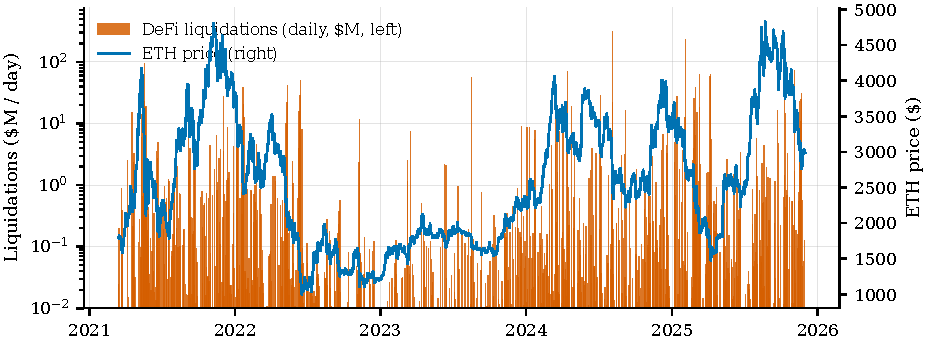
\includegraphics[width=\textwidth]{../paper/figures/fig1_liquidations_timeseries}
\caption{Daily DeFi liquidations (ETH-like collateral, log scale) and the
ETH price, 2021--2025. The flow is sparse, right-skewed, and concentrated
in a handful of stress episodes.}
\label{fig:timeseries}
\end{figure}

\subsection{Data limitations}
\label{sec:data-limits}

The data limitations flagged above are collected here in one place: (1)
hourly aggregation, hence lost within-hour sequencing and short-horizon
bidirectionality; (2) MakerDAO de facto absent; (3) no centralized-exchange
liquidations; (4) ETH-like collateral includes liquid-staking derivatives
but predates and so excludes the liquid-restaking generation, a one-sided
under-count concentrated in 2024--2025;
(5) open interest and funding measured at a single venue; (6) BTC--ETH
co-movement implies the shock is partly a common-crypto stress proxy
(Sections~\ref{sec:deconstruction} and~\ref{sec:discussion}); (7) turnover
denominators used for scale comparisons are industry estimates, partly
inflated by wash trading, and are treated as order-of-magnitude bounds only,
since the liquidation numerator is the only hard number; (8) the window is
post--DeFi-Summer; (9) the dust and exploit filters make the measure
conservative.                % §2  Data (sec:data)
\section{Three Stylized Facts}
\label{sec:stylized}

Before any estimation, three descriptive regularities frame the question.
Together they make the leverage-cycle reading a priori doubtful, which
is why the apparently confirming result of Section~\ref{sec:apparent}
deserves the scrutiny it receives in Section~\ref{sec:deconstruction}.

\paragraph{Fact 1.}
ETH's distribution is downside-asymmetric and fat-tailed, but the asymmetry is market-wide.
Hourly log returns have skewness \SkewEth{} and excess kurtosis \KurtEth{}
(Table~\ref{tab:descriptives}); the worst hour ($\MinRet\%$) is 1.7 times
deeper than the best ($+\MaxRet\%$); and far-extreme counts are
left-heavy, with \FarFiveDown{} hours at or below $-5\%$ against \FarFiveUp{}
at or above $+5\%$ (\FarSevenDown{} versus \FarSevenUp{} at $\pm 7\%$). The
measurement deserves precision, because the 1\% and 5\% \emph{quantiles}
themselves are nearly symmetric ($|p_1|/p_{99} = \QratioOnePct$): the
left-heaviness is a property of the far extremes, not of the moderate
tails. Heavy tails as such are the expected stylized fact
\citep{cont2001,osterrieder2017}, and the \emph{sign} of crypto skewness
varies with the return definition and sample: \citet{liu2021} report
positive skewness in simple returns across major cryptocurrencies, whereas
the hourly log returns studied here skew negative. Two further observations
discipline the interpretation. Negative jumps, a driver of volatility
documented across the major crypto markets \citep{ftiti2021}, are not
specific to ETH, and tail dependence
\emph{across} cryptocurrencies is, if anything, stronger on the upside
\citep{nguyen2020}. So nothing in Fact 1 licenses an attribution of the
asymmetry to DeFi. Figure~\ref{fig:distribution} displays the distribution.

\begin{figure}[t]
\centering
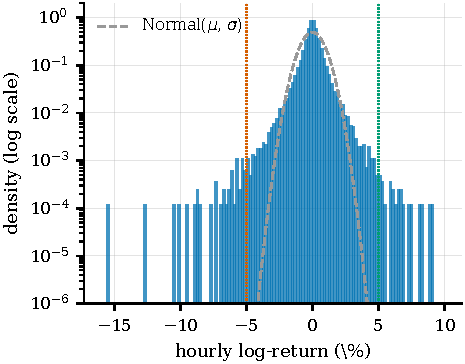
\includegraphics[width=0.55\textwidth]{../paper/figures/fig2_return_distribution}
\caption{Hourly ETH log returns (density, log scale) against a normal
benchmark. Dotted lines mark the $\pm 5\%$ far-extreme thresholds of
Table~\ref{tab:descriptives}.}
\label{fig:distribution}
\end{figure}

\paragraph{Fact 2.}
Liquidations are a mechanical marker of crashes, not evidence of causing them.
Among the worst 1\% of return hours, \PLiqWorstOne\% contain
contemporaneous liquidations, against \PLiqBestOne\% of the best 1\% and
\PLiqAll\% of all hours (Table~\ref{tab:descriptives}, Panel B).
The direction of this co-occurrence is mechanically determined. A price
fall pushes positions below their collateral threshold and triggers
liquidation, which is the protocol design \citep{qin2021,perez2021},
whereas a rally liquidates nothing. This asymmetry therefore
reflects the one-sidedness of the liquidation trigger, not downside
amplification of prices by DeFi. Consistently, \citet{moallemi2024}
document that over 70\% of liquidations occur in the absence of any
downward price jump, and pool-level price impacts of liquidations are small and temporary \citep{tian2025}. Fact 2 is the foundation of the paper's
register: at the hourly grain the liquidation--return relation is
bidirectional at short horizons, so every estimate below is read as
predictive association, never as a causal effect.

\paragraph{Fact 3.}
The observable flow is minute relative to the ETH market.
Median daily DeFi liquidations amount to roughly \SizeMedianShare{} of one percent
of estimated ETH spot-plus-perpetual turnover; the mean is
\SizeShareMean\%; and even the worst liquidation day of the sample reaches
only \SizeShareWorstDay\% (Table~\ref{tab:sizeratio} below reports the full
set). Against the largest reported centralized-exchange liquidation cascade on
record, roughly nineteen billion dollars in a single day
\citep{coinglass2025}, the typical daily flow sits four to six orders of
magnitude lower. The denominators are industry estimates, partly inflated
by wash trading and not peer-reviewed, so these are order-of-magnitude
bounds. But the inequality is wide enough to survive any plausible
rescaling, and the numerator is our own hard extraction. Fact 3 pre-loads the mechanism discussion of
Section~\ref{sec:mechanisms}: whatever the within-pool impact of an
individual liquidation, the aggregate observable flow is small relative to
the market that would need to be moved.

\medskip
\noindent
These three regularities, a real but market-wide asymmetry, mechanically
reverse co-occurrence, and negligible scale, make it doubtful from the
outset that observable DeFi liquidations drive ETH's downside tail. The
remainder of the paper tests that doubt formally: the next section fixes
the specification, Section~\ref{sec:apparent} shows how a naive
quantile analysis nevertheless appears to confirm the leverage-cycle
prediction, and Section~\ref{sec:deconstruction} explains why that
appearance is an artifact of interpretation.      % §3  Stylized facts (sec:stylized)
\section{Empirical Strategy}
\label{sec:method}

\subsection{The estimand}

For each quantile $\tau$ and horizon $h$ we estimate, by local projection
\citep{jorda2005}, the response of the conditional return quantile to the
liquidation shock:
\begin{equation}
\label{eq:qlp}
\QR_{\tau}\!\left(r_{t+1 \to t+1+h} \mid \mathcal{F}_t\right)
 = \beta_h(\tau)\, L_{t-1}
 + \delta_h(\tau)\, \left(L_{t-1} \times \texttt{oi\_high}_t\right)
 + \gamma_h(\tau)' X_t ,
\end{equation}
where $r_{t+1 \to t+1+h}$ is the cumulative ETH return over the $h+1$ hours from $t+1$ to $t+1+h$ (so $h=0$ is the one-hour-ahead return),
$L_{t-1}$ the lagged log-liquidation shock, and $X_t$ the controls of
Section~\ref{sec:method-controls}. The object of interest is
$\beta_h(\tau)$ across $\tau \in \{0.01, 0.05, 0.10, 0.50, 0.90, 0.95\}$
and $h \in \{0, \dots, 24\}$ hours (a nine-quantile grid is reported in the
appendix). Estimation is by quantile regression \citep{koenker1978}; the
estimator and its bootstrap inference follow \citet{han2024}. The reported
grid stops at $\tau = 0.95$; the tail-inference and mirror set additionally
estimates $\tau = 0.99$, so that the one-percent upper tail has a symmetric
counterpart to the one-percent lower tail. Both grids are fixed in the locked
configuration file, so $0.99$ is estimated but not carried into the reported
panels.

The quantile approach is necessary rather than cosmetic, for two reasons.
First, the hypothesis under test, leverage-cycle amplification
\citep{geanakoplos2010,brunnermeier2009}, is a statement about the
\emph{tails} of the return distribution, not its mean. Second, the mean is
empirically silent here: an OLS local projection of returns on the shock
finds nothing at any horizon (point estimate $\approx \OlsLpBetaHzero$ on
impact, HAC $p = \OlsLpPHzero$). This is the Growth-at-Risk logic of
\citet{adrian2019}
transposed to high-frequency crypto returns: tails can respond where the
mean is blind. We note at the outset a tension that
Section~\ref{sec:deconstruction} resolves. \citet{adrian2019} interpret
asymmetric tail sensitivity through conditional skewness;
\citet{carriero2024} show that symmetric conditional distributions, under joint shifts in mean and variance, can produce the same apparent pattern; and \citet{brownlees2021} find that a
plain GARCH rivals quantile-regression Growth-at-Risk out of sample.
Distinguishing those readings is the heart of this paper.

\subsection{Shock definition and timing}
\label{sec:method-shock}

The canonical shock is \emph{raw}: $L_{t-1} = \ln(1 +
\text{liq}^{\text{USD}}_{t-1})$, one-hour lagged
(Section~\ref{sec:data}). Timing is read strictly. ``$h=0$'' is a
one-hour-ahead prediction; within the bucket at $h=-1$, prices and
liquidations co-move mechanically (the reverse-causality zone of Fact 2);
only $h \le -2$ would be a true lead. All claims are therefore
predictive associations.

A second, \emph{orthogonalized} shock (the residual of an OLS regression
of the log flow on contemporaneous and lagged BTC returns, then lagged)
is reserved for the cross-asset placebo (Test A of the robustness battery),
in the ex-ante residualization spirit of \citet{borusyak2022}. The two
definitions preserve sign and significance at every horizon and agree to
within a few percent from six hours out, but diverge at short horizons (the
impact tail coefficient is about 60\% larger under orthogonalization). The
choice between raw and orthogonalized is thus an identification convention
that leaves the symmetry finding and the bound intact, not a claim of
numerical coincidence at every horizon; residualizing at the quantile (rather than by OLS)
is an acknowledged refinement left for future work.

\subsection{Controls and the identification logic}
\label{sec:method-controls}

The regressor set is locked:
$\{L_{t-1},\; L_{t-1}\times\texttt{oi\_high}_t,\; \texttt{oi\_high}_t,\;
r^{\text{BTC}}_t,\; \sigma^{7d}_t,\; \text{funding}_t,\; \text{basis}_t\}$.
The realized-volatility control $\sigma^{7d}_t$ (168-hour rolling standard
deviation) is not a nuisance term: it is central to the identification.
Liquidations raise volatility, and volatility widens \emph{both}
tails symmetrically; the leverage-cycle prediction is specifically
\emph{downside} amplification. Holding $\sigma^{7d}_t$ fixed conditions
$\beta_h(\tau)$ on the \emph{predetermined} volatility state, removing the
confound between the shock and the pre-existing volatility regime. It does
not remove the shock's own forward-volatility response
(Section~\ref{sec:volchannel}). But that response is symmetric, so it cannot
manufacture asymmetry; it is the symmetric residual that the placebo and
the paired tail tests identify directly. The asymmetry tests, not this
control alone, are therefore what separate a real downside shape from a
symmetric scale effect. That a symmetric conditional distribution can
masquerade as downside risk is the demonstration of \citet{carriero2024},
there through joint shifts in mean and variance; the scale-versus-shape
distinction is what quantile regression makes testable
\citep{koenker1982,machado2000}. Realized volatility is preferred to a
GARCH or implied measure because it is observable, model-free, and
predetermined; model-based volatility enters only inside the placebo DGPs
of Section~\ref{sec:deconstruction}, where its model-dependence is the
point.

\subsection{Inference}
\label{sec:method-inference}

Inference proceeds on two tiers. At central quantiles, kernel standard
errors (Hall--Sheather bandwidth) are retained. At tail quantiles
($\tau \in \{0.01, 0.05, 0.95, 0.99\}$), the primary inferential object is
the percentile confidence interval from a moving-block bootstrap with
24-hour blocks \citep{fitzenberger1998,politis1994,gregory2018}, for two
reasons. First, the cumulative left-hand side is overlapping by
construction, so residuals are serially correlated at every $h > 0$
\citep{montiel2021,lusompa2023}; blocks of one day, the maximal horizon,
preserve that dependence. Second, at $\tau = 0.01$ roughly 406
observations sit below the conditional quantile, and the extremal quantile
regression literature shows the asymptotic distribution is non-Gaussian
that far in the tail \citep{chernozhukov2005,chernozhukov2011}, making
kernel inference unreliable: on the exact headline specification, the
bootstrap-to-kernel standard-error ratio at $\tau = 0.01$ ranges from
\SeRatioMin{} to \SeRatioMax{} across horizons
(Appendix Table~\ref{tab:seratio}). All bootstrap results use $1{,}000$
replications with a deterministic multi-level seeding scheme. The MBB block
length does not drive the results: re-running the tail inference at 12-, 36-, and
48-hour blocks leaves every interval and every minimum detectable effect
essentially unchanged (Appendix Table~\ref{tab:blocksens}).

\subsection{The diagnostic battery}
\label{sec:method-battery}

The core methodological contribution is a battery of diagnostics. Each one is
designed to isolate a single confound of the naive reading. What survives all
of them is what we are willing to call a real signal.

\begin{table}[t]
\centering
\caption{Diagnostic tests, one per confound.}
\label{tab:battery}
{\small
\begin{tabular}{p{0.27\textwidth}p{0.21\textwidth}p{0.42\textwidth}}
\toprule
Diagnostic & Confound isolated & Logic \\
\midrule
Symmetric sign-flip placebo & volatility (scale) & does a zero-skew world
with the real volatility path reproduce $\beta(0.01)$ and the left--right
gap? \citep{wu1986,liu1988,davidson2008,carriero2024} \\
Dual permutation nulls & overlap artifact & destroy the shock--return link
(circular shift; innovation reshuffle), keep the cumulative LHS: any
surviving $\beta$ is mechanical \citep{hodrick1992,boudoukh2008,valkanov2003} \\
Tail-exceedance regressions & (the predictor + the symmetry test) & does
the shock predict future tail violations, and equally on both sides?
\citep{engle2004,balcilar2017} \\
Standardized skew tests & scale noise & standardize by predetermined volatility, then
test down-minus-up and the third moment \citep{neuberger2021,farago2023} \\
BTC-outcome placebo & asset specificity & re-run the full QLP with BTC as
the outcome: does the signature replicate on an asset without the
ETH-collateral channel? \\
Equivalence bounds (MDE/TOST) & power & convert ``not found'' into ``we
exclude effects larger than $X$''
\citep{altman1995,ioannidis2017,lakens2017,riesthuis2024} \\
Out-of-sample pinball test & in-sample overfit & does liquidation
information improve rolling-origin tail forecasts against nested and
GARCH benchmarks? \citep{diebold1995} \\
Planted-cascade positive control & power (false negatives) & does the
battery recover a sign-specific downside asymmetry planted at known scale,
and stay silent below it? \\
\bottomrule
\end{tabular}}
\end{table}

Table~\ref{tab:battery} summarizes the battery; applications and results
are in Sections~\ref{sec:deconstruction}--\ref{sec:survives}. The
equivalence step requires a pre-specified smallest effect size of interest
(SESOI). We set it at a one-percentage-point difference in tail-violation
probability between the downside and upside over the span of the shock,
translated into coefficient units under three calibrations of that span
(interquartile, median-to-95th, and 10th-to-90th percentile of the nonzero
shock); the strictest yields \SesoiStrict{} per unit of the log shock. The
one-point threshold is decisional, not statistical. It is the smallest
down-versus-up tail miscalibration a Value-at-Risk desk would act on, not the
smallest the sample can resolve \citep{lakens2017}. One percentage point is
the order at which a shift in the realized 1\% exceedance rate moves a model
across the Basel traffic-light boundary over the standard 250-day backtesting
window. That window is the institutional unit at which tail calibration is
judged by mandate, and we anchor the threshold to it rather than to the far
finer statistical resolution of a forty-thousand-hour sample.

\subsection{Multiple testing and the locked specification}

Bonferroni corrections guard the grid searches: a $\times 12$ family over
the reported $\tau \times h$ cells and a $\times 6$ family over the
quantile grid. The correction family is the set of reported cells itself, the
$\tau \times h$ grid and the quantile grid enumerated in the locked
configuration file before the diagnostic phase, so the family is fixed by the
specification rather than chosen after seeing the diagnostics. The direct shock effect survives both families in full
(12/12 and 6/6); the leverage interaction $\delta_h(\tau)$ fails all six
(0/6). We carry that null forward as it stands, since the interaction was the
specification's embodiment of the leverage-cycle prediction. We read it as a
\emph{detectability} null, not a tight bound (the interaction is imprecisely
estimated; Section~\ref{sec:apparent-crack}), and the paper's quantitative
bounds rest on the asymmetry objects, not on this count. The
corrections guard against noise, not against artifacts, which is exactly why
the battery of Table~\ref{tab:battery} exists.

The specification was locked before the diagnostic phase: every parameter
(quantile grids, horizons, controls, block length, replication counts,
seeds) is fixed in a single configuration file, and every diagnostic is a
flagged auxiliary analysis, never a modification of
Equation~\eqref{eq:qlp}. The full pipeline, from panel construction through
estimation, robustness, diagnostics, and every number, table, and figure in
this paper, regenerates from public data with a one-command replication
package; local smoke runs and the canonical compute environment reproduce
point estimates to three decimals.              % §4  Empirical strategy (sec:method)
\section{The Apparent Result}
\label{sec:apparent}

\subsection{The naive quantile profile}

Table~\ref{tab:qlp} and Figure~\ref{fig:irf} report the headline estimates
of Equation~\eqref{eq:qlp}. On impact, the response of the first percentile
is $\beta_0(0.01) = \BetaQoneHzero$, strongly significant under the
tail-appropriate block-bootstrap inference, while the median barely moves
($\beta_0(0.50) = \BetaMedHzero$). The tail response is
\RatioTailMedImpact{} times the median response. The left tail also appears
to respond more than the right, with $|\beta_0(0.01)|/|\beta_0(0.95)| =
\GapLrImpact$ on impact.

At first reading this is what the leverage-cycle prior\footnote{The
view we deconstruct is actively held, not a strawman built for contrast.
Alongside the leverage-cycle theory cited here it rests on the fire-sale
tradition \citep{shleifer1992}, finds empirical grounding for DeFi in the
leveraging spirals documented by \citet{perez2021} and the systemic
fragility analyzed by \citet{lehar2022}, and is monitored by the official
sector as a financial-stability concern \citep{oecd2023,fsb2023}.} predicts
\citep{geanakoplos2010,brunnermeier2009}: a liquidation shock depresses the
crash quantile of returns far more than the center, and more than the
upside. It is, term for term, the Growth-at-Risk pattern of
\citet{adrian2019}, with the lower tail responding where the mean is blind
(our OLS control regression sees nothing at any horizon). And it is produced
by an established estimator \citep{han2024}, not an exotic one. The
reservation entered below is never about the \emph{existence} of
$\beta$; it is about its \emph{interpretation}.

\begin{table}[t]
\centering
\caption{Quantile local projections: $\beta_h(\tau)$ of cumulative ETH
returns on the liquidation shock.}
\label{tab:qlp}
% GENERATED by scripts/paper/make_tables.py — DO NOT EDIT
% fragment only: wrap in \begin{table} + caption in the manuscript
\begin{tabular}{lcccccc}
\toprule
$\tau$ & $h=0$ & $h=1$ & $h=3$ & $h=6$ & $h=12$ & $h=24$ \\
\midrule
0.01 & -0.032 & -0.087 & -0.105 & -0.160 & -0.241 & -0.213 \\
0.05 & -0.019 & -0.045 & -0.046 & -0.079 & -0.102 & -0.116 \\
0.10 & -0.013 & -0.030 & -0.034 & -0.043 & -0.061 & -0.095 \\
0.50 & 0.002 & 0.006 & 0.010 & 0.014 & 0.032 & 0.038 \\
0.90 & 0.014 & 0.028 & 0.038 & 0.047 & 0.070 & 0.102 \\
0.95 & 0.018 & 0.031 & 0.044 & 0.041 & 0.077 & 0.116 \\
\bottomrule
\end{tabular}

\begin{minipage}{0.92\textwidth}
\vspace{2pt}
{\scriptsize \emph{Notes:} Locked specification (seven regressors,
Section~\ref{sec:method}); $N \approx \Nobs$. Point estimates; tail
inference is by moving-block bootstrap (Figure~\ref{fig:irf} displays the
95\% band on $\tau=0.01$), kernel standard errors being unreliable at
extreme quantiles (Appendix Table~\ref{tab:seratio}).}
\end{minipage}
\end{table}

\begin{figure}[t]
\centering
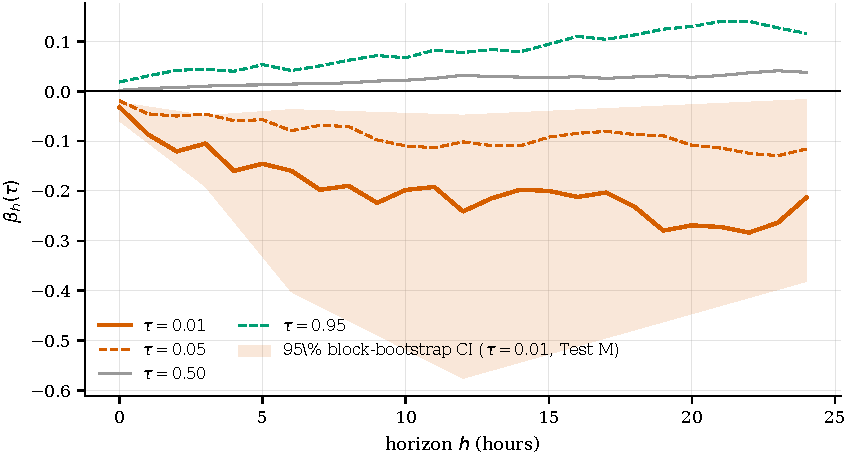
\includegraphics[width=\textwidth]{../paper/figures/fig3_qlp_irf}
\caption{Quantile local-projection responses $\beta_h(\tau)$ with the 95\% block-bootstrap band on $\tau = 0.01$ (headline specification). The fan widens and the lower tail deepens with the horizon.}
\label{fig:irf}
\end{figure}

\subsection{The deepening profile}

The tail coefficient deepens almost monotonically with the horizon:
$\BetaQoneHzero$ on impact, $\BetaQoneHone$ at one hour, $\BetaQoneHtwelve$
at twelve, with a plateau near $\BetaQoneHtwentyfour$ at twenty-four
(Table~\ref{tab:qlp}). An effect that grows as the window lengthens reads
naturally as the footprint of a spiral, the shock propagating and
self-reinforcing, which is the reading a leverage-cycle prior
invites. We flag, without yet arguing, that the left-hand side at $h > 0$
is an overlapping cumulative return, a construction whose tail behavior
under the null deserves dedicated scrutiny, and receives it in
Section~\ref{sec:deconstruction}
\citep{hodrick1992,boudoukh2008,neuberger2021,farago2023}.

\subsection{The apparent robustness}

The pattern checks every box a referee would ask for. The block-bootstrap
band on $\tau = 0.01$ excludes zero at every horizon (on impact
$[\TestMLoHzero, \TestMHiHzero]$; at twelve hours
$[\TestMLoHtwelve, \TestMHiHtwelve]$; at twenty-four
$[\TestMLoHtwentyfour, \TestMHiHtwentyfour]$; $1{,}000$ replications). The
sign and significance survive a battery of conventional robustness checks,
including placebo assets, alternative shock definitions, subperiod and
episode exclusions, and monotonicity across quantiles, reported in
Appendix~\ref{app:robustness}. And the direct effect survives Bonferroni
correction in full: 12 of 12 cells of the reported $\tau\times h$ grid and
6 of 6 of the quantile grid. By the usual standards of empirical asset pricing, this is a
robust result.

Two cautions temper the checklist. Multiple-testing corrections guard
against \emph{noise}, not against \emph{misinterpretation}. Surviving
Bonferroni says the effect is not sampling luck; it does not say the effect
is a downside skew rather than a symmetric volatility response read through
extreme quantiles. And at $\tau = 0.01$ the extremal quantile literature
counsels explicit caution on point estimates
\citep{chernozhukov2005,chernozhukov2011}; tail inference here therefore
rests on interval estimates, from the moving-block bootstrap motivated on
separate grounds in Section~\ref{sec:method-inference}.

\subsection{The leverage interaction}
\label{sec:apparent-crack}

The leverage-cycle story makes a sharper prediction than ``liquidations
depress the tail'': amplification should be \emph{stronger when leverage is
high}. The interaction term $\delta_h(\tau)$, the specification's direct
embodiment of that prediction, is null across the tail-quantile grid. At $\tau = 0.01$ the
bootstrap interval straddles zero at every horizon (on impact
$[\IntCILoHzero, \IntCIHiHzero]$; at twelve hours
$[\IntCILoHtwelve, \IntCIHiHtwelve]$), the sign is unstable across
resamples, and the Bonferroni family verdict is 0 of 6. This is not a
nuance to be excused. The one mechanism-specific term in the regression
fails on the tail grid, while the mechanism-agnostic direct term looks
spectacular. The leverage-cycle reading already has a hole in it.

We are careful about what this null does and does not establish. Unlike the
direct effect, the interaction is estimated with little precision: the
bootstrap interval is wide and its sign flips across resamples, so the
smallest leverage amplification it could detect at conventional power,
\MdeDeltaHzero{} at impact, is a multiple of the direct effect itself,
roughly \MdeDeltaRatioMin{} to \MdeDeltaRatioMax{} times it, not a fraction
of it. The 0/6 verdict
is therefore best read as the \emph{absence of any detectable}
leverage-specific amplification rather than as a tight bound on its
magnitude, a hole in the mechanism story rather than a measured zero. The
decisive, quantified bounds in this paper attach to the symmetric-scale and
down-minus-up asymmetry objects (Section~\ref{sec:survives}), where
standardizing by predetermined volatility cancels the common scale and
sharpens the test; the interaction inherits no such cancellation, which is
why it stays wide. The interaction is, however, not null at the centre of the
distribution: at the median it is significantly negative at the twelve- to
twenty-four-hour horizons ($\delta_{12}(0.50) = \DeltaIxnMedHtwelve$,
$p = \DeltaIxnMedHtwelveP$), so high-leverage hours shift the shock's median
response downward. That is a level effect on the centre of the return
distribution, not the downside-tail amplification the leverage-cycle prior
predicts, and it is orthogonal to the down-minus-up asymmetry this paper
bounds; it is consistent with a liquidation channel that is real and locally
disruptive yet does not aggregate into tail fragility
(Section~\ref{sec:mechanisms}).

\subsection{Summary of the apparent result}

Taken together: a direct effect \RatioTailMedImpact$\times$ the median on
impact, deepening to \BetaQoneHtwelve{} by twelve hours, robust across a
battery of robustness checks, surviving multiple-testing correction in full, and
a mechanism term that is cleanly null. The question that the next
section answers is the one this contrast forces. Is the real, robust
direct effect a genuine \emph{downside} response, or the same symmetric
volatility that thickens \emph{both} tails, misread by a quantile local
projection on overlapping cumulative returns?     % §5  The apparent result (sec:apparent)
\section{Deconstruction}
\label{sec:deconstruction}

\subsection{What must be explained}

Section~\ref{sec:apparent} leaves three facts to explain: a strong negative
$\beta_h(0.01)$ that deepens from \BetaQoneHzero{} to \BetaQoneHtwelve{}
over twelve hours; a tail-to-median ratio of \RatioTailMedImpact{} on
impact; and a left tail that appears to respond more than the right. Three
readings compete. The first is genuine downside-specific amplification, the
leverage-cycle interpretation; the second is a genuine but \emph{symmetric}
volatility channel, misread; the third is a mechanical artifact of the overlapping
cumulative design. We do not adjudicate by assertion. Each alternative is
confronted with a test built to manufacture the stylized fact under
a known null: if the test reproduces the fact, the fact is not a signature
of the first reading. Two distinctions organize the section. The \emph{level} of $\beta$
and the \emph{shape} of the response are separate questions. Level
means the magnitude of $|\beta_h(0.01)|$ (the scale channel of
Section~\ref{sec:method-controls}, tested by the permutation nulls); shape
means the left-minus-right gap $g_h = |\beta_h(0.01)| -
|\beta_h(0.99)|$\footnote{The gap pairs each tail quantile with its
equidistant mirror: $0.01$ with $0.99$, and the headline ratio of
Section~\ref{sec:apparent} pairs $0.01$ with $0.95$. The reporting grid
stops at $0.95$, but $0.99$ is estimated as part of the tail-inference set
(Section~\ref{sec:method-inference}); the headline ratio uses $0.95$ as the
rhetorical object, while the rigorous left-versus-right test below uses the
true mirror $0.99$.} (tested by the placebo). A coefficient can
therefore be genuine in level yet symmetric in shape, and that, we will conclude, is
exactly what the data say. And ETH-specificity is a separate question again, tested by
replacing the outcome altogether.

\subsection{The symmetric placebo}
\label{sec:placebo}

We simulate a world that is symmetric by construction and re-run the exact
estimation kernel on it. Returns are rebuilt as $r^{\text{sim}}_t = m_t \pm
|\hat{\varepsilon}_t|$, where $m_t$ is the fitted conditional mean and the
sign is an independent Rademacher draw, the sign-flip construction of
the wild-bootstrap literature \citep{wu1986,liu1988,davidson2008}. The
simulated world thus has \emph{zero skew by construction} at every point in
time, while preserving the empirical magnitude sequence exactly: the full
fat-tailed, volatility-clustered path of $|\hat{\varepsilon}_t|$, with no
volatility model imposed at all. Because the sign-flip removes asymmetry
while leaving the volatility path untouched, any left--right gap this world
produces is, by construction, what symmetric heteroskedasticity alone
manufactures through extreme quantiles. A gap that the real data
merely matches therefore cannot be evidence of real downside skew. Only the
dependent variable is simulated;
the shock and all controls are the real series. Each of 500 simulated
panels is passed through the identical quantile-LP kernel, and the
statistic of interest is the left--right gap $g_h = |\beta_h(0.01)| -
|\beta_h(0.99)|$. The level of $|\beta|$ is expected to survive (the
volatility path is real, which is the point), so the test bites on the
\emph{asymmetry}, which the design rules out as a property of the data.

The zero-skew world reproduces the observed asymmetry everywhere
(Figure~\ref{fig:placebo}). At twelve hours the real gap
($\GapRealHtwelve$) sits near the center of the placebo distribution
($[\GapBandLoHtwelve, \GapBandHiHtwelve]$); on impact the real gap
($\GapRealHzero$) lies within the symmetric band
($[\GapBandLoHzero, \GapBandHiHzero]$). There is no real impact gap either. Nor is this
verdict an artifact of the band's width. Sweep the placebo's tail
thickness across a variance-preserving family, from thin- to
heavy-tailed, and the real gap stays inside the symmetric band at the data's
own tail thickness and under every heavier tail; it escapes only when the
simulated world is forced thinner-tailed than the data, an artificially
narrow band that under-represents the spread the returns actually carry. A
dose-response sweep of the heteroskedasticity \emph{amplitude} (tracing
the manufactured gap against a tail-thickness parameter) would only
confirm the monotonicity of a mechanism the placebo already exhibits at the
data's own heteroskedasticity, at the cost of an arbitrary parametric family,
and is omitted. A vol-model-scaled variant, in which standardized magnitudes are permuted
across dates and rescaled by a fitted volatility path (a shock-driven
rolling specification and a shock-agnostic GARCH(1,1), two
distinct designs), delivers the same verdict in all fourteen
model-horizon cells. The observed left--right asymmetry is therefore what
symmetric heteroskedasticity looks like through extreme quantiles of
cumulative returns, the mechanism demonstrated for macroeconomic tail risk by \citet{carriero2024}, instantiated here on asset returns. Consistently,
\citet{brownlees2021} find that a symmetric GARCH rivals
quantile-regression tail-risk models out of sample: the scale channel does
the work. One reading discipline applies. Where the placebo occasionally
generates more asymmetry than observed, the correct statement is
that the real gap does not exceed what a zero-skew world generates; the
test is one of non-exceedance, not of equality.

\begin{figure}[t]
\centering
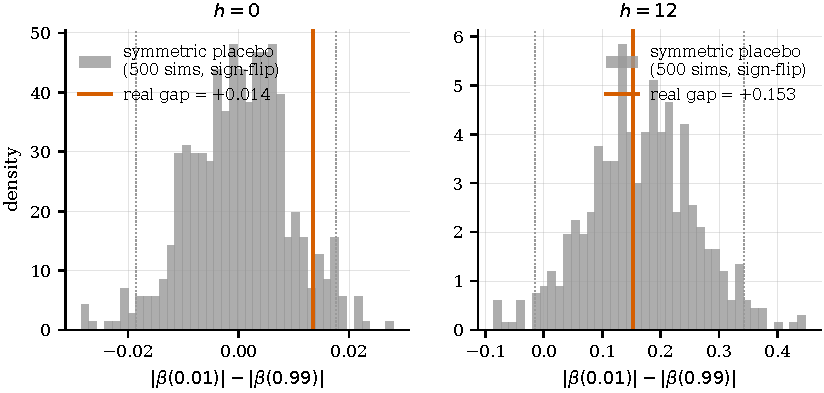
\includegraphics[width=\textwidth]{../paper/figures/fig4_placebo_gap_distribution}
\caption{Distribution of the left--right tail gap $|\beta(0.01)| - |\beta(0.99)|$ across 500 zero-skew sign-flip placebo worlds (grey; dotted lines mark the 2.5th/97.5th percentiles), against the real gap (vertical line), on impact and at twelve hours. The real asymmetry is indistinguishable from what a symmetric world produces.}
\label{fig:placebo}
\end{figure}

\subsection{The permutation nulls}
\label{sec:purenull}

The placebo addresses shape. The level question, whether the deepening
$\beta_h(0.01)$ is a mechanical artifact of the overlapping cumulative design
\citep{hodrick1992,boudoukh2008,valkanov2003}, is answered with two
permutation nulls run at 500 draws each, and reported jointly as a
guard against null-shopping. The conservative null circularly shifts the
shock series, preserving its marginal distribution and autocorrelation
(and the real, heteroskedastic dependent variable) while severing only its
alignment with returns. The coarser null reshuffles the return innovations
themselves, destroying their serial dependence; the two designs bracket
what a ``no information'' world can mean here, and diagnostics of what
each null preserves and destroys are recorded with the artifacts.

Both nulls return the same verdict (Figure~\ref{fig:purenull}). Mechanical
noise accounts for a minority of the observed coefficient at every
horizon: the null-to-real magnitude ratio at twelve hours is
\PnCircHtwelve{} under the conservative null and \PnInnovHtwelve{} under
the coarser one, rising to at most \PnCircHtwentyfour{} at twenty-four
hours. The signed mean of the null distribution is essentially zero
throughout (e.g.\ \PnCircSignedHtwelve{} at twelve hours, against a real
coefficient of \BetaQoneHtwelve): the overlap inflates the
\emph{dispersion} of tail estimates, it does not push them downward.
And the real coefficient lies outside the null band
($[\PnCircQloHtwelve, \PnCircQhiHtwelve]$ at twelve hours) at every
horizon, with permutation $p$-values below $0.005$ through eighteen hours
and \PnCircPermPHtwentyfour{} at twenty-four. The level is
overwhelmingly real.\footnote{The medium-horizon \emph{magnitude} is
separately sensitive to the MakerDAO coverage gap (Appendix~\ref{app:data});
the permutation nulls certify only that the deepening is not a mechanical
artifact of overlap, a distinct question from coverage.} This matters in both
directions. It removes the
artifact reading as a primary explanation, and it sharpens the burden
on interpretation: the coefficient is real, so the question is entirely
what it means.

\begin{figure}[t]
\centering
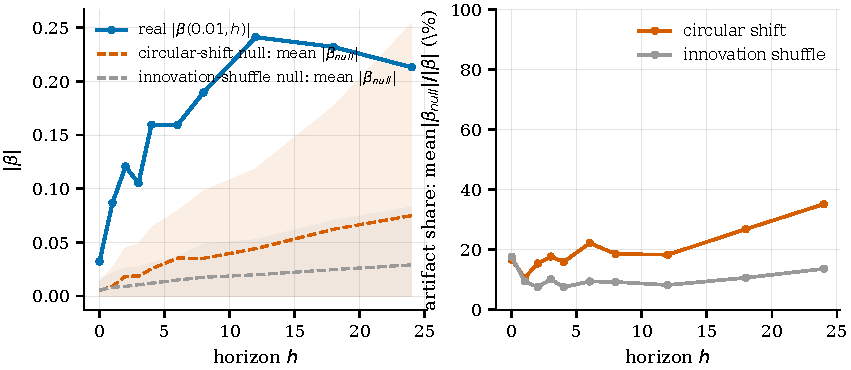
\includegraphics[width=\textwidth]{../paper/figures/fig9_pure_null_dual}
\caption{Dual permutation nulls. Left: the real $|\beta_h(0.01)|$ against
the mean null magnitude under each construction (shaded: null bands).
Right: the null-to-real ratio by horizon, a minority share everywhere,
under both nulls.}
\label{fig:purenull}
\end{figure}

\subsection{The overlap artifact}
\label{sec:overlap}

If the overlapping cumulative construction misleads about \emph{shape}
rather than level, the cleanest demonstration is to remove it. The
exceedance regressions of Section~\ref{sec:survives} use per-period (non-overlapping)
tail-violation indicators; their paired asymmetry $\Delta_h =
\beta^{\text{down}}_h - \beta^{\text{up}}_h$ is null at every horizon
(at twelve hours, $p = \DeltaExcHtwelveP$). Re-running the same
construction on overlapping cumulative returns manufactures a significant
asymmetry at exactly the horizons where the naive reading is most
dramatic ($\Delta_{12} = \DeltaExcCumHtwelve$, $p = \DeltaExcCumHtwelveP$;
Figure~\ref{fig:exceedance}, right panel). Same data, same controls, same
estimator family. The only difference is the overlap. The
horizon-dependent skewness that cumulation fabricates
\citep{neuberger2021,farago2023} is not a theoretical curiosity here; it is
visible in one comparison.

One might worry the null is an artifact of conditioning, that holding the
controls fixed is what suppresses the asymmetry. Re-estimating the effect on
the \emph{marginal} return quantile, by the unconditional-quantile (RIF)
method, answers it. On the density-normalized scale the combined
tail-widening at impact is large (\RifVolWideningImpact), both tails opening
together, the volatility channel again, while the down-versus-up asymmetry
recovered from the same estimates reproduces the conditional exceedance
($\Delta_0 = \DeltaExcImpact$) to machine precision at every horizon. The
agreement is partly algebraic: RIF-OLS with these
controls is the conditional linear-probability model up to the density
factor, so it confirms the null rather than re-deriving it independently.
What the unconditional lens adds is the one distinct object,
the large symmetric widening, and it points the same way.

\subsection{The headline ratio}

The ``\RatioTailMedImpact$\times$'' headline deserves a closer look,
because it is rhetorically the strongest number in
Section~\ref{sec:apparent} and statistically the emptiest. Volatility
widens both tails but does not move the center: $\beta_h(0.50) \approx 0$
is what a scale channel implies (and what the silent OLS mean
regression already said). A tail-to-median ratio with a near-zero
denominator explodes mechanically; it measures ``the median is immobile,''
not ``the downside is special.'' Diverging quantile slopes, the fanning
of Figure~\ref{fig:irf}, are the textbook signature of
heteroskedasticity, not of shape change \citep{koenker1982,machado2000}.
And the correct contrast, left tail against right tail, is the one
the ratio hides: $\beta_{12}(0.05) = \BetaFiveHtwelve$ against
$\beta_{12}(0.95) = \BetaNinetyFiveHtwelve$, both tails moving. At
horizons beyond impact the median itself drifts positive
($\beta_{12}(0.50) = \BetaMedHtwelve$), and the ratio collapses to
\RatioTailMedHtwelve$\times$. The headline number is also
impact-specific.

\subsection{The BTC-outcome placebo}
\label{sec:btc}

A final alternative survives the tests above: perhaps the response is
real and symmetric, and still specifically about ETH's DeFi collateral
channel. The sharpest test replaces the outcome. We re-run the full
quantile local projection, identical shock and horizons, with
Bitcoin returns as the dependent variable (the cross-asset control
becoming ETH's return, by symmetry; BTC has no comparable ETH-collateral
DeFi channel). The ETH signature replicates on Bitcoin in every respect
(Figure~\ref{fig:btc}): $\beta^{\text{BTC}}_0(0.01) = \BtcBetaQoneHzero$
on impact, deepening to $\BtcBetaQoneHtwelve$ at twelve hours, a
near-parallel profile at \BtcOverEthHzero{} of the ETH magnitude on impact
and \BtcOverEthHtwelve{} at twelve hours, with an even more extreme
tail-to-median ratio on impact (\BtcRatioTailMedImpact$\times$, BTC's
median response being essentially zero). The naive signature is therefore
not evidence of an ETH-specific DeFi channel. It is what generic crypto
stress looks like through this lens, on any correlated asset. The residual
claim of ETH specificity is accordingly demoted: BTC carries most of the
signature, and no ETH-specific increment large enough to drive the result
survives. The methodological lesson gains generality, since the
misreading would afflict any asset regressed on any stress-correlated
flow.

\begin{figure}[t]
\centering
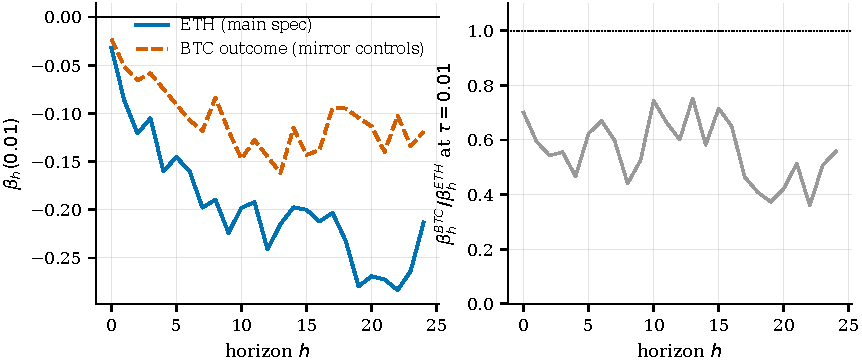
\includegraphics[width=\textwidth]{../paper/figures/fig8_btc_vs_eth}
\caption{BTC-outcome placebo. Left: $\beta_h(0.01)$ profiles, ETH (main specification) and BTC as outcome (mirror controls). Right: the BTC-to-ETH coefficient ratio by horizon. The apparent ``downside-amplification'' signature replicates on an asset without the ETH-collateral channel.}
\label{fig:btc}
\end{figure}

\subsection{The portable detection battery}
\label{sec:lesson}

What is new here, and what is borrowed, should be stated carefully. The
mechanism, symmetric and time-varying volatility producing apparent
downside sensitivity in quantile models, is established in the
macroeconomic Growth-at-Risk setting by \citet{carriero2024}; the overlap
pathologies of long-horizon regressions are classic
\citep{hodrick1992,boudoukh2008,valkanov2003}; scale-versus-shape in
quantile regression goes back to \citet{koenker1982} and
\citet{machado2000}. What is new, to our knowledge, is the
\emph{conjunction} in which all four ingredients meet (asset returns,
overlapping cumulation, quantile local projections, and the extreme tail)
together with a diagnostic battery that detects the trap on real data:
a model-free zero-skew placebo for shape, dual permutation nulls for
level, a per-period-versus-cumulative comparison that exhibits the
artifact directly, a cross-asset outcome placebo for specificity, and a
planted-cascade positive control under which the equivalence apparatus
recovers a downside asymmetry at twice the actionable threshold and stays
silent below it, so the bounded null it returns is power-confirmed, not
power-absent. The lesson travels: any literature that regresses extreme quantiles of
cumulative returns on stress-correlated regressors, and the nascent
empirical DeFi literature is about to be one, can produce
``endogenous fragility'' of this apparent strength from a symmetric
volatility channel.

\subsection{Reconciliation}

The reconciled reading of Section~\ref{sec:apparent} is now complete. In
\emph{level}, $\beta_h(0.01)$ is overwhelmingly genuine: both
permutation nulls leave mechanical noise a minority share, with no signed
bias. In \emph{shape}, the asymmetry is not real. A zero-skew world
reproduces the entire left--right gap at every horizon, the per-period
construction shows both tails loading equally, and the headline ratio is
an artifact of an immobile median. In \emph{specificity}, the signature
replicates on Bitcoin. What the naive analysis detected is a real,
symmetric, generic-crypto volatility response, the second moment
dressed up as downside fragility. What remains to establish is what
survives on the positive side, and how tightly the null can be bounded;
that is Section~\ref{sec:survives}.      % §6  Deconstruction (sec:deconstruction)
\section{What Survives}
\label{sec:survives}

After the deconstruction, the question is no longer whether the apparent
downside amplification is real. As a \emph{downside} effect it is not. The
question is what remains once volatility and the overlap artifact are
accounted for. Three objects survive the battery, and they tell a single
coherent story: a real second-moment channel, a symmetric and
out-of-sample-validated tail predictor, and a null that is not merely
insignificant but \emph{bounded}.

\subsection{The volatility channel}
\label{sec:volchannel}

Regressing forward realized volatility over the $h$-hour window on the
shock and the full control set yields positive, strongly significant
coefficients at every horizon, rising from \VolRespHzero{} on impact to
\VolRespHtwelve{} at twelve hours (per unit of the log-liquidation shock;
an absolute-return measure confirms sign and scale). One unit caveat
applies throughout. The coefficient is percentage points of volatility per
unit of log liquidations, not an elasticity per percent liquidated, so only
the sign and order of magnitude are comparable to the transaction-level
estimates of \citet{oecd2023}, whose direction we replicate and extend from
the conditional mean to the conditional tails. This channel is real,
expected, and mundane. It is also the engine of the entire deconstruction.
It is this symmetric second-moment response that, propagated through
cumulative returns and extreme quantiles, masqueraded as downside
amplification in Section~\ref{sec:apparent}.

\subsection{The tail-risk predictor}
\label{sec:predictor}

In sample, the per-period exceedance regressions (tail-violation indicators in the
CAViaR tradition of \citet{engle2004}, estimated with the full control set,
conditioning on the predetermined volatility state) show the shock loading
positively on \emph{both} tails at every level and horizon
(Figure~\ref{fig:exceedance}, left): on impact at the 1\% level,
$\beta^{\text{down}} = \ExcDownOneHzero$ and
$\beta^{\text{up}} = \ExcUpOneHzero$; at the 5\% level,
\ExcDownFiveHzero{} and \ExcUpFiveHzero{} (all bootstrap intervals exclude
zero). Liquidations predict elevated tail risk on both sides of the
distribution. This two-sided loading has a natural reading in the
microstructure of information: just as a market maker's own quotes can reveal
the direction of their inventory to others (the price-reading channel of
\citet{barzykin2025}), an observable, predetermined flow of forced
deleveraging is a public signal other agents can read. What it reveals is the
magnitude of impending risk rather than its sign, which is why liquidations
forecast elevated violations in both tails symmetrically rather than a signed
downside amplification. To our knowledge this is among
the first quantile-resolution evidence on on-chain forced deleveraging. Adjacent work studies on-chain
flows into means and volatilities, or trading volume across return quantiles
without finding volatility effects \citep{balcilar2017}.

\begin{figure}[t]
\centering
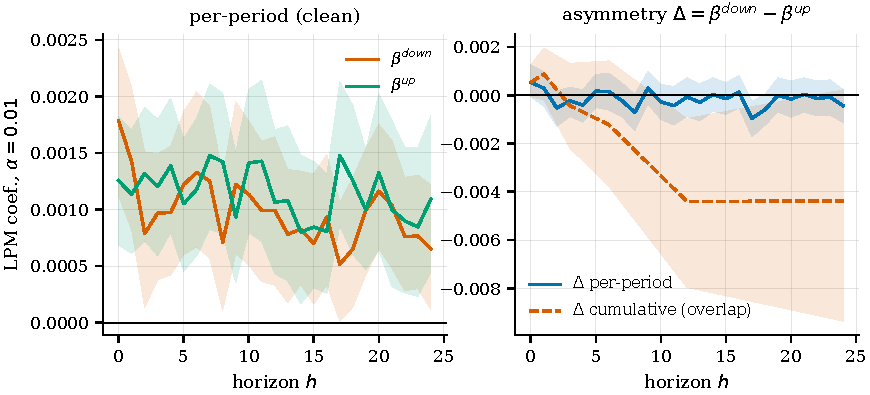
\includegraphics[width=\textwidth]{../paper/figures/fig5_exceedance_symmetry}
\caption{Per-period exceedance coefficients and paired asymmetry. Left: per-period exceedance coefficients at $\alpha = 1\%$, where both tails load positively. Right: the paired asymmetry $\Delta_h$ under the per-period construction (null everywhere) and under the overlapping cumulative construction (a significant asymmetry is manufactured at long horizons), the overlap artifact of Section~\ref{sec:overlap}.}
\label{fig:exceedance}
\end{figure}

An in-sample coefficient, however robust, is not yet a predictor. We use a
rolling-origin evaluation (weekly re-estimation, pinball loss on the
held-out tail forecasts, Diebold--Mariano inference on the loss
differentials \citep{diebold1995}). Adding the liquidation terms to an
otherwise identical quantile model improves tail forecasts directionally in
all twenty nested-QR cells, most not individually distinguishable from zero,
and significantly at both moderate tails at short horizons
(at one hour: \OosSkillFiveHone\% at $\tau = 0.05$,
$p = \OosPFiveHone$; \OosSkillNinetyFiveHone\% at $\tau = 0.95$,
$p = \OosPNinetyFiveHone$; Table~\ref{tab:oos}). These two cells, and a third at a long horizon ($\tau = 0.95$, twenty-four
hours), survive a Benjamini--Hochberg correction across the grid
($\OosNsurviveFDR$ of the twenty do, FDR-adjusted $p = \OosPFiveHoneFDR$ and $\OosPNinetyFiveHoneFDR$;
the 95\% cell survives even the stricter Holm bound), so the surviving
positive finding meets the multiple-testing discipline applied to the
interaction null. The symmetric reading carries out of sample. The boundary
is equally clear. Against a dedicated GARCH(1,1) scale benchmark the picture is deliberately
different: the augmented model does not systematically outperform it, the
short-horizon cells that beat the nested benchmark do \emph{not} beat GARCH
(one, $\tau = 0.95$ at one hour, significantly underperforms it), and the only
cells that beat GARCH are sparse long-horizon ones. That boundary is the point
rather than a concession. The liquidation signal is observable, predetermined, and
exogenous to any price model, so the information it carries is orthogonal and
incremental to the market-state controls a risk desk already tracks: a free
input to add to an existing tail-risk model, not a replacement for one.
Because pinball loss is the objective a quantile VaR forecaster minimizes,
the one-percent reduction at the moderate tails reads directly as a
calibration gain in a one-hour-ahead, on-chain-observable VaR signal,
consistent with the \citet{brownlees2021} finding that symmetric scale
models are formidable tail forecasters. A dollar quantification of that gain
would require position-level data and is left for future work.

\begin{table}[t]
\centering
\caption{Out-of-sample pinball skill of liquidation information (\%),
against a nested quantile benchmark (top panel) and a dedicated GARCH(1,1)
scale model (bottom panel).}
\label{tab:oos}
% GENERATED by scripts/paper/make_tables.py — DO NOT EDIT
% fragment only: wrap in \begin{table} + caption in the manuscript
\begin{tabular}{lccccc}
\toprule
 & $h=1$ & $h=3$ & $h=6$ & $h=12$ & $h=24$ \\
\midrule
\multicolumn{6}{l}{\emph{vs.\ nested QR (no liquidation terms)}} \\
$\tau=0.01$ & 1.41 & 1.03 & 1.10 & 1.18$^{*}$ & 0.81 \\
$\tau=0.05$ & 0.97$^{***}$ & 0.46$^{**}$ & 0.36$^{*}$ & 0.47$^{**}$ & 0.15 \\
$\tau=0.95$ & 0.85$^{***}$ & 0.56$^{**}$ & 0.37$^{*}$ & 0.26 & 0.60$^{***}$ \\
$\tau=0.99$ & 0.51 & 0.54 & 1.11$^{**}$ & 0.03 & 0.03 \\
\midrule
\multicolumn{6}{l}{\emph{vs.\ GARCH(1,1) benchmark}} \\
$\tau=0.01$ & 0.33 & -0.78 & 0.51 & 2.14$^{*}$ & 1.59 \\
$\tau=0.05$ & -0.61 & -0.61 & -0.16 & -0.19 & 1.00 \\
$\tau=0.95$ & -1.47$^{**}$ & -1.07 & -0.59 & -0.50 & 1.42$^{**}$ \\
$\tau=0.99$ & -0.44 & 0.41 & 1.38 & 0.29 & 2.51$^{*}$ \\
\bottomrule
\end{tabular}

\begin{minipage}{0.92\textwidth}
\vspace{2pt}
{\scriptsize \emph{Notes:} Rolling-origin forecasts of the per-period
$\tau$-quantile of ETH returns; expanding window, weekly refits, 97
re-estimations, $\sim$16{,}200 test hours. Skill $= 1 -
L_{\text{full}}/L_{\text{bench}}$ in percent; stars from Diebold--Mariano
tests with HAC variance ($^{*}$ $p<0.10$, $^{**}$ $p<0.05$, $^{***}$
$p<0.01$). Source: \texttt{oos\_predictive.csv}.}
\end{minipage}
\end{table}
\subsection{The bounded null}
\label{sec:boundednull}

Net of volatility, downside-specific
amplification is not economically significant, and what is excluded is
quantified in three steps.

\paragraph{(i) Raw symmetry.}
The paired asymmetry $\Delta_h = \beta^{\text{down}}_h -
\beta^{\text{up}}_h$, estimated on the same block resamples so the
difference is properly paired, is statistically indistinguishable from
zero at every horizon and tail level (Table~\ref{tab:nullbound}, Panel A):
at the 1\% level on impact, $\Delta_0 = \DeltaExcImpact$
($p = \DeltaExcImpactP$), with unstable signs across levels and horizons.

\paragraph{(ii) The standardized residual.}
Standardizing returns by predetermined volatility before forming the
asymmetry measures does not remove a scale bias. A symmetric scale
effect, predetermined or shock-induced, cancels in any down-minus-up
difference, which is why the raw paired contrast in (i) is already null.
What standardizing does is reduce the scale noise that masks a small shape
residual, raising power. At the moderate tail the residual is null
($p = \SkewTailFiveP$ at the 5\% level). At the extreme tail a small
positive residual becomes statistically detectable: $\beta = \SkewTailOne$ ($p = \SkewTailOneP$) on the 1\% tail
indicator, with a winsorized third-moment regression also significant
($\ZthreeWinsor$). This sharpening, not any new channel, is why the
residual surfaces here but not in the lower-powered raw contrast or in the
Section~\ref{sec:placebo} placebo, which compared the raw, vol-dominated
gap. Net of volatility, the extreme downside is therefore not
literally perfectly symmetric. The question that matters is whether
the detectable residual is large enough to matter.

\paragraph{(iii) The bound.}
It is not. Converting the bootstrap intervals into minimum detectable
effects and equivalence tests \citep{lakens2017,riesthuis2024} against the
pre-specified smallest effect size of interest
(Section~\ref{sec:method-battery}), the exceedance asymmetry at the 1\%
level is equivalent to negligible under all three calibrations of
the shock span, including the strictest (MDE at 80\% power
\MdeEightyExc{}, below the strictest SESOI of \SesoiStrict); the residual
itself is equivalent-to-negligible under two calibrations and borderline
under the strictest (Table~\ref{tab:nullbound}, Panel C, and
Figure~\ref{fig:mde}).\footnote{Read as a continuous function of the
smallest effect size rather than at the three pre-registered calibrations
alone, the verdict does not turn on the choice of span: the exceedance
$\Delta$ is equivalent-to-negligible for every SESOI above \SesoiEquivExc{},
at or below all three locked spans, so it clears even the strictest;
and the residual for every SESOI above \SesoiEquivSkew{}, which sits just
above the strictest span and hence above only it, leaving the strictest
calibration as the single inconclusive reading already noted.} The resulting
statement is the paper's central
quantitative claim: we can rule out a downside-specific tail
asymmetry larger than roughly \MdeEightyExc{} per unit of the log
liquidation shock, evidence of absence at the economically relevant
scale, not mere absence of evidence \citep{altman1995,ioannidis2017}. The moderate tails (5\%, 10\%) are underpowered for
strict equivalence, so the strong bound lives at the 1\% level. That is
also where the residual lives, so it is the bound that matters. The scope is narrow by design: the asymmetry the introduction documents is a far-extreme property, the $\pm 5\%$ and $\pm 7\%$ counts of Section~\ref{sec:stylized}, near the $0.1\%$ tail that an hourly panel cannot resolve, so the bound concerns one-percent-tail downside specificity rather than amplification of that far-extreme asymmetry. And the
third-moment regression is excluded from the equivalence exercise on
unit grounds (a third moment is not a probability gap).

\paragraph{The positive control.}
A bound is only as credible as the battery's ability to find what it
claims to exclude, so we ran the full equivalence apparatus on a synthetic
series into which a sign-specific downside cascade was planted at known
scale. The headline object behaves as a calibrated instrument
should: a planted asymmetry at half the smallest effect size of interest
is returned as equivalent-to-negligible and goes undetected (point
estimate \PosCtrlDeltaHalf{}); at the threshold itself the verdict is
inconclusive (\PosCtrlDeltaOne{}); and at twice the threshold the
asymmetry is recovered as non-negligible, its interval lying beyond the
band (\PosCtrlDeltaTwo{}). Because the standard error is a within-panel
block bootstrap anchored to the same \MdeEightyExc{} rather than to the
simulation budget, this graduation is a property of the data's information
content, not of how long we ran the planting. The equivalence apparatus
therefore detects a genuine, sign-specific downside asymmetry of
roughly twice \SesoiStrict{} and is correctly silent below it. That is
what converts the all-negative real result from ``we found nothing'' into
the sharper ``there is nothing at or above that scale to find.'' This certifies
the power of the equivalence apparatus, the object that claims the bound; the
symmetric placebo is deconstructive rather than a claim of absence and owes
no such demonstration, though the same planting also escapes its band at and
above that scale. One limit should
be stated. The cascade is planted in the units the tests read, so the
control certifies the battery's operating characteristics at a known,
now economically anchored, effect size rather than re-detecting a skew that
emerges from a structural process; a fully emergent cascade, a calibrated
leverage spiral, is left for future work.

\begin{table}[t]
\centering
\caption{Paired asymmetry, standardized skew, and equivalence verdicts.}
\label{tab:nullbound}
% GENERATED by scripts/paper/make_tables.py — DO NOT EDIT
% fragment only: wrap in \begin{table} + caption in the manuscript
\begin{tabular}{lcccc}
\toprule
\multicolumn{5}{l}{\emph{Panel A: paired exceedance asymmetry $\Delta_h = \beta^{\text{down}}_h - \beta^{\text{up}}_h$, $\alpha = 1\%$ (per-period)}} \\
$h$ & $\Delta$ & 95\% CI & & $p$ \\
\midrule
0 & 0.00053 & [-0.00006, 0.00125] & & 0.110 \\
1 & 0.00029 & [-0.00045, 0.00097] & & 0.428 \\
3 & -0.00023 & [-0.00088, 0.00033] & & 0.466 \\
6 & 0.00015 & [-0.00062, 0.00090] & & 0.694 \\
12 & -0.00007 & [-0.00087, 0.00072] & & 0.844 \\
24 & -0.00044 & [-0.00112, 0.00023] & & 0.234 \\
\midrule
\multicolumn{5}{l}{\emph{Panel B: vol-standardized skew tests (h=0)}} \\
measure & $\beta$ & 95\% CI & & $p$ \\
\midrule
tail indicator, $\tau{=}5\%$ & 0.00043 & [-0.00075, 0.00158] & & 0.446 \\
tail indicator, $\tau{=}1\%$ & 0.00071 & [0.00018, 0.00126] & & 0.012 \\
winsorised $z^3$ & -0.02930 & [-0.04391, -0.01479] & & $<$0.001 \\
\midrule
\multicolumn{5}{l}{\emph{Panel C: equivalence (TOST) verdicts vs.\ SESOI spans}} \\
object & MDE$_{80}$ & IQR span & strict span & $p_{10}{\to}p_{90}$ \\
\midrule
exceedance\_delta ($\alpha{=}$0.1 (h=0)) & 0.00231 & equiv. & inconcl. & inconcl. \\
exceedance\_delta ($\alpha{=}$0.05 (h=0)) & 0.00171 & equiv. & inconcl. & equiv. \\
exceedance\_delta ($\alpha{=}$0.01 (h=0)) & 0.00094 & equiv. & equiv. & equiv. \\
skew\_test (skew\_tail05) & 0.00166 & equiv. & inconcl. & equiv. \\
skew\_test (skew\_tail01) & 0.00077 & equiv. & inconcl. & equiv. \\
skew\_test (z3\_winsor) & 0.02081 & n/a & n/a & n/a \\
\bottomrule
\end{tabular}

\begin{minipage}{0.92\textwidth}
\vspace{2pt}
{\scriptsize \emph{Notes:} Panel A: paired moving-block bootstrap
($1{,}000$ replications, 24-hour blocks). Panel B: returns standardized by
predetermined 7-day realized volatility. Panel C: MDE at 80\% power and
TOST equivalence verdicts against the three SESOI calibrations of
Section~\ref{sec:method-battery}. Sources: \texttt{exceedance\_paired.csv},
\texttt{skew\_test.csv}, \texttt{mde\_equivalence.csv}.}
\end{minipage}
\end{table}

\begin{figure}[t]
\centering
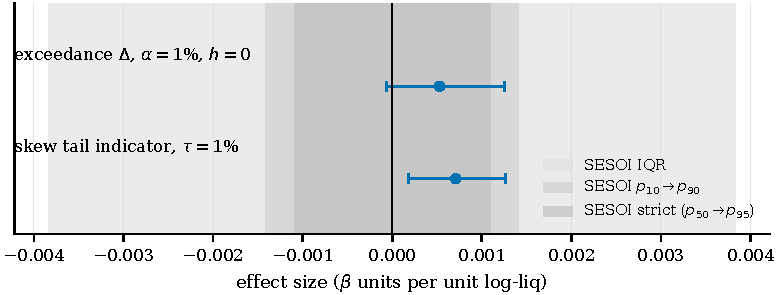
\includegraphics[width=\textwidth]{../paper/figures/fig7_mde_equivalence}
\caption{Point estimates and 95\% intervals for the two 1\%-tail asymmetry objects against the three SESOI bands. The residual is statistically detectable yet economically negligible.}
\label{fig:mde}
\end{figure}

\subsection{Stability}
\label{sec:stability}

The surviving objects are not the artifact of one episode or one tuning
choice. Splitting the sample in half leaves the tail profile essentially
unchanged. Excising the August 2024 episode, the largest liquidation
event in the sample, preserves about seventy percent of the
twelve-hour deepening ($\BetaQoneHtwelveLoo$ against \BetaQoneHtwelve)
while the paired asymmetry stays null in every subsample
(Table~\ref{tab:subsample}). The block-bootstrap inference, and hence the
equivalence bound itself, is insensitive to the block length: re-running
the critical cells at 12-, 36-, and 48-hour blocks moves the MDE by less
than a tenth of its value (Appendix Table~\ref{tab:blocksens}). One
sample nuance is reported. The small positive impact
tilt in $\Delta_0$ is concentrated in the first half of the sample
(2021--2023, the Terra/FTX era) and sits in the
contemporaneous-reverse-causality zone, vanishing at $h \ge 1$ and in the
later subsample.

\begin{table}[t]
\centering
\caption{Subsample stability: the tail profile and the paired asymmetry.}
\label{tab:subsample}
% GENERATED by scripts/paper/make_tables.py — DO NOT EDIT
% fragment only: wrap in \begin{table} + caption in the manuscript
\begin{tabular}{lcccccc}
\toprule
 & \multicolumn{4}{c}{$\beta_h(0.01)$} & \multicolumn{2}{c}{$\Delta$ at $h{=}12$} \\
\cmidrule(lr){2-5}\cmidrule(lr){6-7}
Subsample & $h=0$ & $h=6$ & $h=12$ & $h=24$ & estimate & MDE$_{80}$ \\
\midrule
Full sample & -0.032 & -0.160 & -0.241 & -0.213 & -0.00007 & 0.00112 \\
First half & -0.030 & -0.175 & -0.229 & -0.214 & -0.00005 & 0.00157 \\
Second half & -0.037 & -0.174 & -0.292 & -0.096 & 0.00017 & 0.00148 \\
Excl.\ Aug-2024 & -0.032 & -0.127 & -0.171 & -0.165 & -0.00002 & 0.00107 \\
\bottomrule
\end{tabular}

\begin{minipage}{0.92\textwidth}
\vspace{2pt}
{\scriptsize \emph{Notes:} $\beta_h(0.01)$ point estimates per subsample;
$\Delta$ at $h{=}12$ with its 80\%-power MDE from the paired bootstrap.
``Excl.\ Aug-2024'' drops a window around 2024-08-05 extended backward by
the maximal horizon, so the episode contaminates neither regressors nor
outcomes. Source: \texttt{subsample\_stability.csv}.}
\end{minipage}
\end{table}

\subsection{What we do not claim}
\label{sec:noclaim}

The guardrails. We do not claim that liquidations
\emph{cause} volatility or tail risk: at short horizons the relation is
bidirectional, and every estimate is a predictive association. We do not
claim the downside effect is literally zero: a 1\% residual is detectable;
we claim it is negligible and \emph{bounded}. Symmetrically, the residual
is not evidence of downside specificity: it is isolated (absent at the
5\% level and in the raw exceedance contrast), below the smallest effect
size of interest, and non-excluded rather than established. We do not
claim OECD-style elasticities, only sign and order of magnitude. And
we do not claim out-of-sample dominance over dedicated volatility models,
only incremental information. What we do claim is the conjunction:
a real, symmetric, bounded second-moment channel, validated in and out
of sample.       % §7  What survives (sec:survives)
\section{Mechanisms}
\label{sec:mechanisms}

Sections~\ref{sec:apparent}--\ref{sec:survives} established an empirical
fact: net of volatility, observable DeFi liquidations do not amplify ETH's
downside tail to any economically significant degree. This section
rationalizes that fact through market structure. The aim is not to
re-estimate it, but to explain why an economist should not have expected
otherwise at the observable DeFi scale. The argument is a beam, not a proof.
No single channel demonstrates the null on its own, and the four are ordered
by evidentiary weight, from the load-bearing channel (size) to the modifier
(oracle). Each bounds one link in the hypothetical leverage-cycle chain,
from liquidation to directional fire sale to permanent price impact to
aggregate spiral, and the register stays descriptive throughout. The
liquidation channel is real and locally disruptive. It raises volatility, as
Section~\ref{sec:volchannel} confirms; it is only too small and too
efficiently cleared to aggregate into a directional downside loop.

\subsection{Size of the liquidation flow}
\label{sec:size}

For a liquidation flow to imprint downside amplification on ETH's
\emph{aggregate} return distribution, it must be material relative to the
turnover that forms that distribution. It is not. In the normal regime the
median daily flow is on the order of \SizeMedianShare{} of one percent of
ETH spot-plus-perpetual turnover (centralized-exchange reported), a rounding error; the mean is
\SizeShareMean\%; and even the worst day of the entire sample reaches only
\SizeShareWorstDay\% (Table~\ref{tab:sizeratio}). Against the largest reported single-day
centralized-exchange liquidation cascade on record, roughly nineteen
billion dollars on 10 October 2025 \citep{coinglass2025}, the typical
daily DeFi flow sits four to six orders of magnitude lower, and the
whole-sample cumulative total amounts to roughly \SizeTotalVsCascade\% of
that single cascade day. A flow this
many orders of magnitude below the venue where a reflexive spiral
plausibly lives (Section~\ref{sec:discussion}) cannot, at the observable
scale, be a material aggregate contributor to ETH's crash quantile. In
aggregate-market terms the hourly shock the quantile projection sees is
negligible, and that is what predicts the null.

\begin{table}[t]
\centering
\caption{Size of the DeFi liquidation flow relative to ETH turnover and to
centralized-exchange cascades.}
\label{tab:sizeratio}
% GENERATED by scripts/paper/make_tables.py — DO NOT EDIT
% fragment only: wrap in \begin{table} + caption in the manuscript
\begin{tabular}{lc}
\toprule
 & Share (\%) \\
\midrule
Mean daily DeFi liq.\ / daily ETH turnover & 0.0032 \\
Median daily DeFi liq.\ / daily ETH turnover & 0.0000 \\
Worst day (2024-08-05) / daily ETH turnover & 0.67 \\
Worst 7 days / 7-day ETH turnover & 0.10 \\
Worst day / Oct-2025 CEX-perp cascade ($\sim$\$19bn) & 1.62 \\
Whole-sample total / Oct-2025 single-day cascade & 13.3 \\
\bottomrule
\end{tabular}

\begin{minipage}{0.92\textwidth}
\vspace{2pt}
{\scriptsize \emph{Notes:} Numerator is our measured flow (the hard
number); denominators are industry turnover estimates
\citep{coingecko2024annual,coingecko2024perps} and a reported cascade
magnitude \citep{coinglass2025}, partly inflated by wash trading
\citep{gan2022} and not peer-reviewed, hence order-of-magnitude bounds. The inequality is wide enough to survive any
plausible rescaling of the denominator. Source: \texttt{size\_ratio.csv}.}
\end{minipage}
\end{table}

The inequality is wide, three to four orders of magnitude, wide enough to
survive deflating the wash-inflated denominators entirely (the numerator
is our own hard extraction; the caveat is detailed at the table). The flow
is also concentrated in a single episode (August 2024). This is why the
median, not the mean, carries the argument, and why we compare the
typical flow to a cascade rather than the outlier day to a cascade.
Agent-based work on DeFi lending finds systemic default rates below a
tenth of a percent even at ten times observed
volatility \citep{chaudhary2022},
and the ecosystem's lending base is itself non-monotone, peaking near
\$45 billion in late 2021 and falling to roughly \$15 billion by mid-2023
\citep{bertomeu2024}. ``Small'' is
not only our empirical finding but what a model of on-chain lending
predicts under stress.

\subsection{Clearing}
\label{sec:clearing}

Even a small flow could imprint directionality if it discharged as a fire
sale, with inventory sold under pressure, in size, into a falling market. The
architecture of DeFi liquidation rules this out for the modal case.
Liquidations are absorbed by well-incentivized liquidators
\citep{qin2021}; over seventy percent of liquidable positions are
liquidated immediately, and eighty-five percent of liquidable collateral
clears within two blocks \citep{perez2021}, leaving no overhang to drain
gradually into the price. And the modal liquidation is not a crash but a
drift in position health. \citet{moallemi2024} document that over
seventy percent of liquidations occur in the absence of any downward price
jump. The central mode of DeFi liquidation is non-directional; the
directional episodes are the tail, not the body. Toxic liquidation spirals
do exist as a mechanism \citep{warmuz2022},
but they are a conditional tail phenomenon (illiquid collateral, deep
undercollateralization), not the modal case, and they do not contradict
the rapid clearing of the typical liquidation.

\subsection{Absorption and price impact}
\label{sec:absorption}

The next link requires the selling pressure to move the market price and
stay there. Automated-market-maker depth and arbitrage absorb and reverse
it instead. The measured price impact of a DeFi liquidation is minuscule, on the order of $0.05\%$ on Aave and $0.01\%$ on Maker at the block level, and temporary
\citep{tian2025}. On the largest AMM, \citet{leharparlour2025} document the absence of long-lived arbitrage opportunities, so a pool-level displacement is corrected rather than propagated into a persistent move in aggregate ETH. The most serious counterweight is the
permanent price impact documented by \citet{lehar2022}, with spillover as
far as centralized venues. But their own evidence bounds its reach for our
asset, in three steps. The flagship contagion in their data runs through
an illiquid collateral token, not through deep ETH; the arbitrage they
document reverses the transient component; and their heavier tails are
explicitly two-sided, with no quantile or asymmetry test. That is a
level-impact result, not an aggregate downside-amplification one. For deep,
hourly ETH, the aggregate footprint is dominated by the symmetric volatility
channel of Sections~\ref{sec:deconstruction}--\ref{sec:survives}, not by a
directional translation of the distribution.

\subsection{Oracle decoupling}
\label{sec:oracle}

The final link would require a transient on-chain price move to feed back
into the aggregate market through the liquidation system itself. DeFi
oracles are largely centralized-exchange-anchored and smoothed: they
aggregate from external venues and are, in the words of the OECD study,
oblivious to small price changes \citep{oecd2023}. A transient
DEX deviation does not mechanically trigger a fresh liquidation wave priced
off that deviation, so there is no small-move price-oracle-liquidation
feedback loop. We place this channel last because its sign is
design-conditional. The same oracle linkage is, in other configurations,
itself a contagion channel, the broader oracle-design problem of
\citet{caldarelli2020}.
For small transient moves on a deep asset, smoothing and anchoring decouple
and attenuate; the oracle-as-cascade channel manifests on large moves of
illiquid assets, consistent with the illiquid-token flagship of
Section~\ref{sec:absorption}. The net effect is in our favor for ETH at the
hourly grain, with the acknowledgment that the reverse mechanism
exists, which is why this is a modifier and not a load-bearing channel.

The adversarial limit of this design-conditional channel is a liquidator who
does not passively receive the oracle price but actively moves it.
\citet{sadeghi2026} study profitable oracle manipulation that triggers
liquidations on constant-product markets, a form of oracle-extractable value,
and identify the transaction-fee conditions under which it becomes
economically unviable. This is the precise micro-mechanism through which a
liquidation-to-price loop could operate on chain, and a theoretical force that
already bounds it. Our result bounds it from the data side: the hourly
equivalence bound of Section~\ref{sec:boundednull} limits the asymmetric
imprint such strategies, were they prevalent on deep ETH, leave in the
aggregate tail, while staying silent on their block-level profitability, which
an hourly panel cannot resolve. The active-liquidator premise is also ours;
the flow we measure is cleared by agents who choose when to act.

\subsection{Synthesis}

The channel is real and raises volatility (Section~\ref{sec:volchannel}), but
too small relative to aggregate ETH turnover (Section~\ref{sec:size}) and too
efficiently cleared (Sections~\ref{sec:clearing}--\ref{sec:oracle}) to
aggregate into a directional downside loop in the observable on-chain channel. The null of
Section~\ref{sec:survives} does not rest on this beam; it is established
empirically and bounded by equivalence. But the beam makes it
intelligible rather than surprising, in order of evidentiary weight: size
(load-bearing, a hard number), then clearing, then absorption, then the
design-conditional oracle modifier. The account is size-contingent. It explains why the channel does not aggregate
\emph{today}, not that it never could, a conditionality
Section~\ref{sec:discussion} takes up.          % §8  Mechanisms (sec:mechanisms)
\section{Scope, Mediation, and Limitations}
\label{sec:discussion}

\subsection{Perimeter}
\label{sec:scope}

What we tested is the observable on-chain channel. A reflexive
leverage-cycle spiral, in the strict sense, plausibly lives on the
centralized perpetual-futures venue, a compartment we do not observe and
therefore neither test nor refute. Our null is not a denial of
centralized-exchange cascades. It is a result about a different object, three
to four orders of magnitude smaller. The scale gap carries this reading. The
typical daily DeFi flow is four to six orders of magnitude below the largest
single-day centralized cascade on record (roughly nineteen billion dollars,
October 2025; Section~\ref{sec:size}), and the largest crashes of the period (Terra, FTX,
October 2025) are uniformly attributed to centralized, perpetual, or systemic
dynamics, never to on-chain DeFi. We are deliberate about the evidentiary
status of that attribution. The weight of evidence favors the centralized
venue, but the causal claim is associative on both sides: event studies,
connectedness measures, and practitioner magnitudes, the very class of
non-identified evidence this paper otherwise declines. The formulation we
prefer is that the centralized venue is the most plausible locus, not an
established cause, and that our DeFi design cannot adjudicate it. The
supporting magnitudes are labeled as event-study and practitioner figures
throughout, and the measured on-chain price impact remains minuscule and temporary \citep{tian2025}, real locally but too small to aggregate.

\subsection{The null in the crypto leverage-effect debate}
\label{sec:mediation}

The field is split. In spot data at lower frequencies the leverage effect
is inverted or absent \citep{baur2018,aharon2023}, while the cascade
narrative, in which liquidations drive the downside, lives in a different
venue, frequency, and jump regime. Our null is the tail-response counterpart
of the inverted-or-absent spot effect, transposed to a new object: net of
volatility, the DeFi shock predicts large up-moves and large down-moves
equally. It is not in tension with the cascade results, which inhabit an
intraday, jump-driven, centralized regime that an hourly on-chain shock does
not capture. The reconciling axis is the decomposition of \citet{huang2022},
in which the diffusive component behaves conventionally while jumps invert, so
the net sign flips with the mix. That is why spot and cascade findings coexist
without contradiction. Our contribution to the debate is one clean empirical
point that sits squarely in the both-tails-respond-more-than-the-mean camp
\citep{ando2022}. We do not adjudicate the true sign of the crypto leverage
effect; we place our null within it. One apparent counter deserves a direct
word. Cross-coin tail dependence is, if anything, stronger on the
\emph{upside} \citep{nguyen2020}, but that is co-dependence across coins, not
a single asset's response to a shock, and it is consistent with our finding of
no downside specificity.

\subsection{Scope of the null}
\label{sec:caution}

The null must be stated precisely. At the observable on-chain scale and over
this period, there is no economically significant downside amplification. That
is not the same as saying there is none, or that there will be none. The
conditional is explicit: \emph{if} the DeFi share of crypto leverage were to
grow materially, the channel \emph{could} become aggregate-relevant. The
weight of that statement is carried by three legs, size
(Section~\ref{sec:size}), mechanism
(Sections~\ref{sec:clearing}--\ref{sec:oracle}), and the official-sector
consensus that DeFi is not yet systemic but bears watching as it grows
\citep{fsb2023,aramonte2021,imf2021,ecb2022}, never by the whisper. The
conditionality is not rhetorical: on-chain leverage \citep{heimbach2024} and
cross-protocol interconnection \citep{badev2023} are each time-varying, and
the ecosystem's measured fragility moves with them \citep{bertomeu2024}. This is why we bound the null
rather than assert a zero. An equivalence bound
(Section~\ref{sec:boundednull}) excludes only a downside asymmetry larger than
roughly \MdeEightyExc{} per unit of shock, which is what makes the null
respectable and falsifiable rather than a bare failure to reject
\citep{altman1995,ioannidis2017}.

The one-percent whisper bounded in Section~\ref{sec:boundednull} is, in
addition, governed at $\tau = 0.01$ by a non-Gaussian limiting distribution
that makes standard inference unreliable to begin with
\citep{chernozhukov2005,chernozhukov2011}. That is one more reason it does not
carry the conclusion, which rests on size, mechanism, and consensus.

\subsection{Limitations}
\label{sec:limitations}

We list the limitations, say why each is one, and state what was done about
it. \emph{(1) Hourly aggregation.} The shock is aggregated to the hour, so
within-hour sequencing is lost and the impact hour mixes trigger and
consequence; we adopt a predictive register and read across horizons, but
no tick-level sequencing is available. \emph{(2) BTC--ETH co-movement.} The
impact response replicates on Bitcoin (Section~\ref{sec:btc}:
$\beta^{\text{BTC}}_0(0.01) = \BtcBetaQoneHzero$ against
$\BetaQoneHzero{}$ for ETH), so the shock is partly a common-crypto stress
proxy rather than purely ETH-specific; the cross-asset placebo is precisely
the diagnostic for this, and the result is what motivates retiring the
specificity claim rather than defending it. \emph{(3) Short-horizon reverse
causality.} \PLiqWorstOne\% of the worst-1\% hours contain contemporaneous
liquidations against \PLiqBestOne\% of the best, so a crash mechanically
triggers liquidations and the short-horizon relation is bidirectional. Hence
the non-causal register, with the one-hour lag and horizon reading as
mitigation. \emph{(4) No centralized exchange.} The perimeter is on-chain
only, so the plausible locus of the spiral is structurally out of reach.
\emph{(5) Mean, not quantile, residualization.} The orthogonalized shock is
the residual of an OLS, not a quantile, regression. We acknowledge this as a
refinement, with the raw in-regression controls serving as the canonical
channel and the orthogonalized shock reserved for the placebo.
\emph{(6) Estimated denominators.} The size ratio rests on
centralized-reported, partly wash-inflated turnover figures, so it is an
order-of-magnitude bound; the numerator is the only hard figure, and the
inequality survives one to two orders of rescaling. \emph{(7) No structural
identification.} Every estimate is a predictive association; converting them
to causal statements would require exogenous variation in liquidation
timing, the most immediate direction for future work. Limitations (1)--(3)
bound causality, (4) bounds scope, and (5)--(7) bound precision; none
invalidates the beam, and together they fix the perimeter of the claim.          % §9  Scope, limitations (sec:discussion)
\section{Conclusion}
\label{sec:conclusion}

This paper began with a real puzzle and a plausible prior. Ethereum's hourly
returns carry a marked downside tail asymmetry, the textbook leverage-effect
explanation is absent or inverted in crypto, and the field falls back on the
liquidation cascade of the leverage cycle, a mechanism that DeFi, alone
among markets, records transaction by transaction. A naive quantile local
projection appears to confirm the prior in full: a first-percentile response
\RatioTailMedImpact{} times the median on impact, deepening with the horizon,
robust across a battery of robustness checks, surviving multiple-testing correction.

A battery of diagnostics overturns that reading without overturning the
estimate. The coefficient is genuine in level. Both permutation nulls
leave mechanical overlap a minority share, with no signed bias. But its
apparent downside specificity does not survive. A symmetric, zero-skew placebo
reproduces the entire left--right tail gap at every horizon; the per-period
construction shows both tails loading equally; the headline ratio is an
artifact of an immobile median; and the whole signature replicates when
Bitcoin is substituted as the outcome. What the naive analysis detected is a
real but symmetric volatility channel, generic to crypto stress, dressed
up as downside fragility. This is the trap that symmetric heteroskedasticity sets
for quantile projections on overlapping cumulative returns, here sprung on
real data where the naive answer looked spectacular.

What survives is modest and worth having. Liquidations are a real,
symmetric predictor of ETH tail risk, in and out of sample. The effect is
incremental to
a nested quantile benchmark, not a replacement for a dedicated scale model;
the volatility
channel they drive confirms and extends the existing transaction-level
evidence to the conditional tails; and, net of volatility, the one-percent-tail
exceedance asymmetry (down minus up) is bounded below the smallest effect
size of interest under all three calibrations of the shock span, including the
strictest, so we can \emph{exclude} downside-specific amplification larger than
roughly \MdeEightyExc{} per unit of the log-liquidation shock. That is evidence of
absence at the economically relevant scale for the one-percent-tail
exceedance-asymmetry object under the stated calibrations of the shock span,
not a bare failure to reject. The small standardized residual at the one-percent tail is statistically
detectable but economically negligible, clearing two of the three calibrations
and borderline under the strictest, and it does not carry the conclusion.

The takeaway is bounded on every side. At the observable on-chain scale and
over this period, DeFi liquidations do not amplify ETH's downside tail
beyond their symmetric volatility effect; they nonetheless predict tail
risk, symmetrically; and a naive quantile local projection overreads that
symmetric volatility as directional fragility. This is not no effect: the
volatility channel is real. The short-horizon relation is bidirectional, so
the finding is not causal. It does not refute centralized-exchange cascades,
which our design cannot observe. And it does not claim that ETH's asymmetry
is fictional. That asymmetry is real; the observable DeFi channel simply adds no
downside-specific amplification to it, net of volatility.
The null is size-contingent: if the DeFi share of crypto leverage grows
materially, the channel could become aggregate-relevant, and the bound bears
re-examination as that share moves.

Four directions follow. We ran an unconditional-quantile (RIF) cross-check
(Section~\ref{sec:deconstruction}); because RIF-OLS is here algebraically tied
to the conditional model, a fully \emph{independent} unconditional
estimator would test the artifact from a separate angle. An identification
strategy
isolating exogenous variation in liquidation timing, whether an adjustable-rate
instrument or residualization at the quantile rather than the mean, would
license the causal statements this paper declines. And centralized
perpetual-futures data would let one test the spiral where it plausibly
lives, outside our perimeter. And broadening the on-chain liquidation panel
beyond the currently indexed lending protocols, to MakerDAO and DAI-vault
liquidations and to liquid-restaking collateral (Appendix~\ref{app:data}),
would close the two coverage gaps whose direction we can bound but not
eliminate here. The contribution we claim is correspondingly
sized: a reproducible on-chain liquidation panel, a portable methodological
caution that symmetric volatility masquerades as fragility in naive quantile
projections, a bounded null against a popular directional prediction, and a
symmetric tail-risk predictor, executed and stress-tested in full.
          % §10 Conclusion (sec:conclusion)

\section*{Declaration on the use of generative AI}
\label{sec:ai-declaration}

This project made substantial use of generative artificial intelligence:
large language models of the Anthropic Claude family (the Opus and Fable
generations, 2026), operated through an agentic coding interface with
multi-agent orchestration, under my direction and subject to my review at
every stage. Their role spanned several parts of the work: discovering and
organising the related literature and assembling the bibliography; proposing
diagnostic and robustness strategies, analytical framings, and candidate
interpretations; scaffolding and drafting analysis and packaging code;
executing the pre-committed estimation pipeline to regenerate the deposited
artifacts; building the verification and reproducibility infrastructure of
the replication package; and drafting and revising targeted passages of the
manuscript. Throughout, I treated these tools as fallible research aids
rather than as sources of authority, and subjected their output to a
verification protocol commensurate with their documented failure modes.

The integrity of the results does not rest on trust in that assistance. The
research question, the locked specification, the identification and
inference strategy, the data sources and their construction, and every
modelling and interpretive decision are my own; the specification was locked
before the diagnostic phase. No reported quantity was estimated by a
language model. All estimates derive from my seeded, deterministic pipeline,
which the assistant executed only to regenerate the committed artifacts; the
regenerated output was verified identical to my originals at reporting
precision, and every in-text numerical macro is byte-matched by a
non-regression guard. Two points warrant note. First, the size shares in
Table~\ref{tab:sizeratio} reflect a change of denominator basis that I
decided and the assistant implemented: deterministic arithmetic over
author-verified industry constants, not estimation, isolated and verified to
move exactly those quantities, with the prior convention retained as an
alternative row. Second, quantities quoted from primary sources were
inserted only after verbatim checking against those sources. Correctness is
therefore established by reproduction rather than by provenance: a single
command re-derives every table and figure from the deposited data on a fresh
clone, the guard confirms that all reported numbers are unchanged after any
code change, and AI-assisted modifications were accepted only when the
guard, the test suite, and a byte-level comparison of independently
regenerated artifacts agreed that the scientific content was unchanged.

The characteristic failure mode of language-model assistance is text that is
fluent but unsupported, and it was treated accordingly. The verification
layer identified and removed several fabricated or mis-attributed citations,
reworded or cut statements that could not be traced to a primary source or
to a re-executable computation, and caught coding errors before they reached
the results; I report this as evidence that verification was both necessary
and applied. The build automation, verification apparatus, and
data-acquisition scripts of the replication package are likewise
substantially AI-authored under my direction and approved by me, and the
committed result files were regenerated under a pinned deterministic
environment. These models do not meet the criteria for authorship. I
reviewed and approved all content and assume sole responsibility for this
paper, including any remaining errors.
      % unnumbered: generative-AI disclosure

\bibliography{references}

\clearpage
\appendix
\section{Robustness Battery}
\label{app:robustness}

The conventional robustness battery referenced in
Section~\ref{sec:apparent} comprises a cross-asset placebo (the
orthogonalized shock applied to XRP and DOGE returns, neither used as
ETH-collateral), alternative shock definitions (raw versus
BTC-orthogonalized), subperiod and crisis-episode exclusions, a
monotonicity test across quantiles, and the exact-specification bootstrap
band of Figure~\ref{fig:irf}. The sign and tail significance of
$\beta_h(0.01)$ and $\beta_h(0.05)$ survive throughout, while the leverage
interaction is null in every variant. This is the pattern of
Section~\ref{sec:apparent-crack}. The full battery and its companion
metadata are in the replication package (\texttt{robustness\_*.csv}).

\paragraph{Dual permutation nulls.}
The two nulls of Section~\ref{sec:purenull} are reported jointly, with their
preservation diagnostics, in
\texttt{pure\_\allowbreak null\_\allowbreak circular\_\allowbreak shift\_\allowbreak by\_\allowbreak horizon.csv} and
\texttt{pure\_\allowbreak null\_\allowbreak innov\_\allowbreak shuffle\_\allowbreak by\_\allowbreak horizon.csv}. The conservative
circular-shift null preserves the shock's marginal distribution and
autocorrelation exactly (verified in the metadata) while severing its
alignment with returns; the innovation-reshuffle null destroys the return's
serial dependence (its absolute-return autocorrelation falls from
its empirical value to essentially zero). Both yield a minority artifact
share at every horizon (\PnCircHtwelve{} and \PnInnovHtwelve{} at twelve
hours), with a signed null mean indistinguishable from zero
(\PnCircSignedHtwelve{} under the conservative null), and the real
coefficient outside the null band throughout. Both constructions are small,
and neither produces a signed downward bias.

\paragraph{Nine-quantile grid.}
The main text reports the six-quantile grid
$\{0.01,\allowbreak 0.05,\allowbreak 0.10,\allowbreak 0.50,\allowbreak 0.90,\allowbreak
0.95\}$; the nine-quantile grid (adding
$0.25$, $0.75$, $0.99$) is provided in \texttt{quantile\_\allowbreak lp\_\allowbreak results\_\allowbreak 9q.csv}
and yields the same qualitative profile, with the $0.99$ upside mirror used
for the left--right gap statistic of Section~\ref{sec:placebo}.           % Robustness battery, dual nulls, 9q grid
\clearpage
\section{Tail Inference}
\label{app:inference}

\paragraph{Same-specification standard-error ratio.}
The case for bootstrap inference at the tail
(Section~\ref{sec:method-inference}) rests on a same-specification
comparison. We take the bootstrap standard error from the exact headline-spec
bootstrap and the kernel standard error from the same table, at
$\tau = 0.01$ (Table~\ref{tab:seratio}). The ratio ranges from
\SeRatioMin{} to \SeRatioMax{} across horizons. This compares like with like.
A cross-specification comparison would instead conflate the standard-error
gap with differences in scale, controls, and shock definition.

\begin{table}[t]
\centering
\caption{Kernel versus bootstrap standard errors, same specification,
$\tau = 0.01$.}
\label{tab:seratio}
% GENERATED by scripts/paper/make_tables.py — DO NOT EDIT
% fragment only: wrap in \begin{table} + caption in the manuscript
\begin{tabular}{lccc}
\toprule
$h$ & kernel SE & bootstrap SE & ratio \\
\midrule
0 & 0.0057 & 0.0094 & 1.65 \\
3 & 0.0229 & 0.0362 & 1.58 \\
6 & 0.0344 & 0.0931 & 2.71 \\
12 & 0.0404 & 0.1346 & 3.33 \\
24 & 0.0465 & 0.0930 & 2.00 \\
\bottomrule
\end{tabular}

\begin{minipage}{0.85\textwidth}
\vspace{2pt}
{\scriptsize \emph{Notes:} Bootstrap standard error from the
exact-specification bootstrap; kernel standard error from the main
table. Source: \texttt{se\_ratio\_nb07.csv}.}
\end{minipage}
\end{table}

\paragraph{Block-length sensitivity.}
The 24-hour block length of the moving-block bootstrap is the maximal
horizon, the natural choice for the overlap structure. Nothing in our results
turns on it. Table~\ref{tab:blocksens} reports the 80\%-power minimum
detectable effect for the paired one-percent asymmetry, the object that
drives the equivalence bound, at block lengths of 12, 24, 36, and 48
hours. The bound moves by less than a tenth of its value across the range.
By construction the 24-hour column reproduces the corresponding cells of the
main exceedance table exactly, a built-in cross-check that the two run on
identical machinery.

\begin{table}[t]
\centering
\caption{Block-length sensitivity of the equivalence bound (MDE at 80\%
power, $\Delta$ at $\alpha = 1\%$).}
\label{tab:blocksens}
% GENERATED by scripts/paper/make_tables.py — DO NOT EDIT
% fragment only: wrap in \begin{table} + caption in the manuscript
\begin{tabular}{lcccc}
\toprule
$h$ & block $=12$h & block $=24$h & block $=36$h & block $=48$h \\
\midrule
0 & 0.00096 & 0.00094 & 0.00089 & 0.00091 \\
1 & 0.00101 & 0.00101 & 0.00096 & 0.00097 \\
3 & 0.00087 & 0.00087 & 0.00087 & 0.00088 \\
6 & 0.00113 & 0.00109 & 0.00097 & 0.00096 \\
12 & 0.00108 & 0.00114 & 0.00112 & 0.00114 \\
24 & 0.00102 & 0.00097 & 0.00099 & 0.00101 \\
\bottomrule
\end{tabular}

\begin{minipage}{0.85\textwidth}
\vspace{2pt}
{\scriptsize \emph{Notes:} Per-period paired bootstrap, $1{,}000$
replications. The 24-hour column reproduces the main exceedance results.
Source: \texttt{block\_sensitivity.csv}.}
\end{minipage}
\end{table}            % block-length sensitivity + same-spec SE ratio
\clearpage
\section{Construction of the Liquidation Measure}
\label{app:data}

The liquidation series is extracted from Dune Analytics query
\texttt{6912877}, versioned in the replication package, over the
open-source Spellbook tables \texttt{lending.borrow} (debt leg) and
\texttt{lending.supply} (collateral leg), across all EVM chains and lending
protocols indexed at extraction time. This appendix records the
construction decisions that materially affect the primary regressor. The
full query is in the package.

\paragraph{Pre-aggregation before the join.}
An event-level join of the debt and collateral legs on transaction produces
a Cartesian product for transactions containing multiple debt and multiple
collateral events. This pattern is common in bundled liquidation bots, and it
inflates totals. The query pre-aggregates each leg by transaction before
joining, eliminating the inflation by construction. The correction revised
the 2024 and 2025 aggregate volumes downward by roughly fourteen and thirty
percent respectively relative to a naive join, while pre-2024 aggregates
moved by less than a quarter of a percent.

\paragraph{Primary measure.}
The primary variable is the hourly sum of debt forcibly repaid in USD,
zero-filled on hours without qualifying liquidations, entered as
$L_{t-1} = \ln(1 + \text{liq}^{\text{USD}}_{t-1})$ with a one-hour lag. The
seized-collateral leg is retained as a robustness alternative. The two
measures correlate above 0.97, and the choice changes the headline
coefficient by less than three percent in log space.

\paragraph{Collateral filter.}
Only liquidations seizing ETH-like collateral are kept, using the symbol set
\{WETH, ETH, stETH, wstETH, rETH, cbETH, sfrxETH, ETHx\}, so the measure
isolates the ETH leverage channel. Liquid-staking derivatives are included,
so the collateral is ETH-like in the broad sense. A depeg of a staking
derivative could in principle inject non-pure-ETH liquidations, a rare
event we note for completeness.

\paragraph{Exclusions.}
Three exclusions are applied on top of the structural filters. Positions
with absolute debt below five dollars are dropped, removing a cluster of
roughly 75{,}000 micro-events in September 2025 linked to bot activity that
is immaterial in dollar terms. UwuLend liquidations from June 2024 onward
are dropped to exclude an exploit-driven hour reporting an implausible
volume attributable to on-chain exploit movements combined with pricing
errors on illiquid tokens. Euler liquidations during the March--April 2023
hack window are dropped; Euler v2, a distinct protocol launched in 2024, is
retained. A small number of hours in late 2025 carry anomalous
collateral-to-debt ratios from oracle pricing of illiquid tokens; these are
economically invisible in the debt-repaid measure.

\paragraph{Coverage caveats.}
MakerDAO, historically the largest on-chain liquidator, sits outside the
Spellbook lending schema (a CDP architecture) and is de facto absent, so the
measure understates total on-chain deleveraging, most severely in 2021. No
centralized-exchange liquidations enter. The query was executed once, on a
single date; a future re-execution may differ marginally if the Spellbook
tables are updated.

\paragraph{Sensitivity to the MakerDAO gap.}
Because the MakerDAO omission is the largest coverage gap, we bound its
effect by an actual re-fit rather than an assumption. We inflate the observed
liquidation series by a missing-Maker share $m$ (up to a punitive $m=0.5$)
and re-estimate the locked specification, placing the missing mass three
ways: proportional to currently-active hours, on stress-adjacent zero hours,
and weighted toward high open-interest (leverage) hours. The shock
coefficient's sign is preserved under every allocation and horizon. At impact
its magnitude moves by at most \MakerLevelImpactPct\%, but at twelve hours the
leverage-weighted infill (the largest-displacement allocation, since Maker
auctions cluster in high-leverage, falling-price hours) attenuates the
deepening by up to \MakerLevelMediumPct\%. Both displacement figures are the
maximum over the defensible allocation range $m \le 0.25$; the punitive
$m=0.5$ end of the sweep changes neither sign nor significance. The
medium-horizon magnitude is therefore coverage-sensitive. The bounded object is not: the per-period exceedance
asymmetry at the 1\% level stays within \MakerExcOverSesoi{} of the smallest
effect size of interest under every allocation, and shrinks toward zero under
the leverage-weighted and stress-adjacent infills, so a more complete measure
would tighten rather than overturn the null.    % Dune query, filters, exclusions

\end{document}
